%%%%%%%%%%%%%%%%%%%%%%%%%%%%%%%%%%%%%%%%%
% Arsclassica Article
% LaTeX Template
% Version 1.1 (10/6/14)
%
% This template has been downloaded from:
% http://www.LaTeXTemplates.com
%
% Original author:
% Lorenzo Pantieri (http://www.lorenzopantieri.net) with extensive modifications by:
% Vel (vel@latextemplates.com)
%
% License:
% CC BY-NC-SA 3.0 (http://creativecommons.org/licenses/by-nc-sa/3.0/)
%
%%%%%%%%%%%%%%%%%%%%%%%%%%%%%%%%%%%%%%%%%

%----------------------------------------------------------------------------------------
%	PACKAGES AND OTHER DOCUMENT CONFIGURATIONS
%----------------------------------------------------------------------------------------

\documentclass[
10pt, % Main document font size
letterpaper, % Paper type, use 'letterpaper' for US Letter paper
twoside, % One page layout (no page indentation)
%twoside, % Two page layout (page indentation for binding and different headers)
headinclude,footinclude, % Extra spacing for the header and footer
BCOR5mm, % Binding correction
]{scrartcl}

%%%%%%%%%%%%%%%%%%%%%%%%%%%%%%%%%%%%%%%%%
% Arsclassica Article
% Structure Specification File
%
% This file has been downloaded from:
% http://www.LaTeXTemplates.com
%
% Original author:
% Lorenzo Pantieri (http://www.lorenzopantieri.net) with extensive modifications by:
% Vel (vel@latextemplates.com)
%
% License:
% CC BY-NC-SA 3.0 (http://creativecommons.org/licenses/by-nc-sa/3.0/)
%
%%%%%%%%%%%%%%%%%%%%%%%%%%%%%%%%%%%%%%%%%

%----------------------------------------------------------------------------------------
%	REQUIRED PACKAGES
%----------------------------------------------------------------------------------------

\usepackage[
nochapters, % Turn off chapters since this is an article        
beramono, % Use the Bera Mono font for monospaced text (\texttt)
eulermath,% Use the Euler font for mathematics
pdfspacing, % Makes use of pdftex’ letter spacing capabilities via the microtype package
dottedtoc % Dotted lines leading to the page numbers in the table of contents
]{classicthesis} % The layout is based on the Classic Thesis style

\usepackage{arsclassica} % Modifies the Classic Thesis package

\usepackage[T1]{fontenc} % Use 8-bit encoding that has 256 glyphs

\usepackage[utf8]{inputenc} % Required for including letters with accents

\usepackage{lineno} %Line Numbers
\usepackage{setspace} %Define Line Spacing

\usepackage{filecontents}

%\usepackage{matlab-prettifier}

\usepackage[framed,numbered,autolinebreaks]{mcode}

%\lstset{
%	style              = Matlab-editor,
%	basicstyle         = \mlttfamily,
%	escapechar         = ",
%	mlshowsectionrules = true,
%}

\usepackage{graphicx} % Required for including images
\graphicspath{{figures/}} % Set the default folder for images
\usepackage{wrapfig}

\usepackage{tikz}
\usepackage{pgfplots}
\pgfplotsset{compat=1.12}
\usepackage{tikz}
\usetikzlibrary{external}
\usetikzlibrary{decorations.shapes}
\tikzexternalize[optimize=false,prefix=cache/]
%\tikzset{external/force remake}
\newlength\figheight
\newlength\figwidth 

\usepackage{booktabs}
\usepackage{array,multirow}

\usepackage{hyperref}
\usepackage{nicefrac}
\usepackage{units}
\usepackage{siunitx}
%\usepackage{sistyle}

%\usepackage{enumitem} % Required for manipulating the whitespace between and within lists
\usepackage{enumerate}

\usepackage{lipsum} % Used for inserting dummy 'Lorem ipsum' text into the template

%\usepackage{subfigure} % Required for creating figures with multiple parts (subfigures)
\usepackage[justification=centering]{caption}
\usepackage{subcaption}

\usepackage{amsmath,amssymb,amsthm} % For including math equations, theorems, symbols, etc
\usepackage{varioref} % More descriptive referencing

\usepackage[left=1.5in,right=1.5in,top=1.75in,bottom=1.75in]{geometry}

\usepackage{url}

\usepackage{mathabx}

\usepackage[backend=biber,style=numeric,firstinits=true,citestyle=numeric]{biblatex}

\addbibresource{bibliography.bib}


%----------------------------------------------------------------------------------------
%	THEOREM STYLES
%---------------------------------------------------------------------------------------

\theoremstyle{definition} % Define theorem styles here based on the definition style (used for definitions and examples)
\newtheorem{definition}{Definition}

\theoremstyle{plain} % Define theorem styles here based on the plain style (used for theorems, lemmas, propositions)
\newtheorem{theorem}{Theorem}

\theoremstyle{remark} % Define theorem styles here based on the remark style (used for remarks and notes)

%----------------------------------------------------------------------------------------
%	HYPERLINKS
%---------------------------------------------------------------------------------------

\hypersetup{
%draft, % Uncomment to remove all links (useful for printing in black and white)
colorlinks=true, breaklinks=true, bookmarks=true,bookmarksnumbered,
urlcolor=webbrown, linkcolor=black, citecolor=black, % Link colors
pdftitle={Assignments}, % PDF title
pdfauthor={\textcopyright}, % PDF Author
pdfsubject={}, % PDF Subject
pdfkeywords={}, % PDF Keywords
pdfcreator={pdfLaTeX}, % PDF Creator
pdfproducer={LaTeX with hyperref and ClassicThesis} % PDF producer
}


%--------------------------------------------------------------------------------------
% OTHERS
%--------------------------------------------------------------------------------------
\usepackage{times}%Uncomment if you want to use Times New Roman Font in Document

\newcommand*{\setiwonafont}{\fontfamily{iwona}\selectfont}

% Degree symbol
\newcommand{\degr}{\textsuperscript{\(\circ\)}}

% sections
\titleformat{\section}
{\relax}{\textsc{\MakeTextLowercase{\bfseries\large\thesection}}}{3em}{\bfseries\Large}

% subsections
\titleformat{\subsection}{\relax}{\textsc{\MakeTextLowercase{\textbf{\thesubsection}}}}{1em}{\bfseries\normalsize\itshape} % Include the structure.tex file which specified the document structure and layout

\hyphenation{Fortran hy-phen-ation} % Specify custom hyphenation points in words with dashes where you would like hyphenation to occur, or alternatively, don't put any dashes in a word to stop hyphenation altogether

%--------------------------------------------------------------------------------------
%	TITLE AND AUTHOR(S)
%--------------------------------------------------------------------------------------

%\title{\normalfont{Development of a Boat Traffic Prediction Model Using an Artificial Neural Network}} % The article title
 
\author{\large{W. Rossell$^1$, Y. Ozeren$^2$, H. Yasarer$^3$}} % The article author(s) - author affiliations need to be specified in the AUTHOR AFFILIATIONS block

\date{} % An optional date to appear under the author(s)


\usepackage{rotating} %To display tables in landscape

\usepackage{fixltx2e}
\usepackage{xcolor}
\def\SPSB#1#2{\rlap{\textsuperscript{\textcolor{black}{#1}}}\SB{#2}}
\def\SP#1{\textsuperscript{\textcolor{black}{#1}}}
\def\SB#1{\textsubscript{\textcolor{black}{#1}}}


\doublespacing

\begin{document}
	\begin{singlespace}
\begin{center}	
	
\textbf{\huge{Development of a Boat Traffic Prediction Model Using an Artificial Neural Network}}\\
\vspace{1cm}
\large{W. Rossell\SP{1}, Y. Ozeren\SP{2}, H. Yasarer\SP{3}}
\vspace{1cm}
%----------------------------------------------------------------------------------------



%\begin{document}

%--------------------------------------------------------------------------------------
%	HEADERS
%----------------------------------------------------------------------------------------

\renewcommand{\sectionmark}[1]{\markright{\normalfont{#1}}} % The header for all pages (oneside) or for even pages (twoside)
\renewcommand{\subsectionmark}[1]{\markright{\thesubsection~#1}} % Uncomment when using the twoside option - this modifies the header on odd pages
\lehead{\mbox{\llap{\small\thepage\kern1em\color{halfgray} \vline}\color{halfgray}\hspace{0.5em}\bfseries\rightmark\hfil}} % The header style

\pagestyle{scrheadings} % Enable the headers specified in this block

%----------------------------------------------------------------------------------------
%	TITLE, TABLE OF CONTENTS & LISTS OF FIGURES AND TABLES
%----------------------------------------------------------------------------------------
%	\vspace{-1cm}
%	\maketitle % Print the title/author/date block
	
	\normalsize \SP{1} Graduate Research Assistant, University of Mississippi - National Center for Computational Hydroscience and Engineering, 243 South Oxford Center, University MS 38677, USA wrossell@ncche.olemiss.edu \\\SP{2} Research Professor, University of Mississippi - National Center for Computational Hydroscience and Engineering, 229 South Oxford Center, University MS 38677, USA yozeren@ncche.olemiss.edu 
	\\\SP{3} Assistant Professor, University of Mississippi - Civil Engineering Department, 106 Carrier Hall University MS 38677, USA, hy@olemiss.edu\\	
		
	\vspace{0.75cm}
	\end{center}
%	\setcounter{tocdepth}{2} % Set the depth of the table of contents to show sections and subsections only
%	
%	\tableofcontents % Print the table of contents
%	
%%	\listoffigures % Print the list of figures
%	
%%	\listoftables % Print the list of tables

%----------------------------------------------------------------------------------------
%	ABSTRACT
%----------------------------------------------------------------------------------------
\numberwithin{equation}{section}
\thispagestyle{empty} %Leaves out the first page number

 % This section will not appear in the table of contents due to the star (\section*)
\textbf{Abstract:}Riverbank erosion is a major concern to neighboring inhabitants and the surrounding environment. Boat generated waves can significantly contribute to riverbank erosion in navigable rivers and waterways. Waves created by high-speed vessels can have wave heights large enough to cause significant damage to the riverbanks. A preliminary step to predicting the impact of boat generated waves is to predict local boat traffic. In this study, 8 models for predicting boat traffic along a reach of the Connecticut River were created using a Feed-Forward Artificial Neural Network, considering different combinations of a variety of inputs. Wave data was collected using four capacitance type wave staffs installed at three sites along the study reach, and processed in a deterministic identification model to define boat traffic counts. Weather conditions were categorized using time-lapse videos recorded at the study sites. Other variables for the development of the boat traffic prediction models were the month of the year, day of the month, day of the week, river stage, water depth, logger location, and measured temperature and precipitation data collected at a nearby weather station in Amherst, MA. 7 models were constructed to predict daily boat traffic. 1 model was constructed to predict hourly boat traffic for comparison. This paper presents a comparison of results and the performance of these various models.
\\
\\
\\
\textbf{Keywords:}Artificial Neural Networks, Machine Learning, Boat-Generated Waves, River Bank Erosion, Boat Traffic Prediction

\end{singlespace}
%----------------------------------------------------------------------------------------
%	AUTHOR AFFILIATIONS
%----------------------------------------------------------------------------------------

%{\let\thefootnote\relax\footnotetext{* \textit{Department of Biology, University of Examples, London, United Kingdom}}}
%
%{\let\thefootnote\relax\footnotetext{\textsuperscript{1} \textit{Department of Chemistry, University of Examples, London, United Kingdom}}}

%----------------------------------------------------------------------------------------

\newpage % Start the article content on the second page, remove this if you have a longer abstract that goes onto the second page
\linenumbers

%----------------------------------------------------------------------------------------
%	Problem 1
%----------------------------------------------------------------------------------------

\section{Introduction}\label{sec:Intro}

%\numberwithin{equation}{section}
\large

Bank erosion is a natural occurrence that can be observed over time in rivers and streams. While many causes of erosion exist, wave action provides a significant contribution to shoreline erosion and the induction of embankment failure \cite{ozeren2016boat}. Wave action can be generated by many natural causes, such as wind and gravity, but waves can also be created by the passing of a high-speed vessel. During a study in the Kenai River, Alaska, undertaken by United States Army Corps of Engineering, Environmental Research and Development Center, these short term boat-generated waves were shown to be capable of transmitting energy equal to as much as 59\% of the energy of  natural streamflow \cite{maynord2008boat}. This study also states that future increase in boat traffic could cause major alteration to river and streambank erosion levels. 

Due to the increasing number of recreational vessels that are owned and used, the amount of bank erosion attributed to boat-generated waves produced by the increase in traffic has become a more significant concern in navigable rivers and waterways \cite{simon2016boat}. In order to predict further change in embankment erosion levels, the trend of increasing boat-traffic must first be predicted. As such, this study sought to produce and compare various boat-traffic prediction models using a Feed-Forward Artificial Neural Network (ANN) with the back-propagation-of-error algorithm. ANN is a computational system derived from a process that uses externally provided information to estimate values of interest. These inputs are functionally independent variables, and these outputs are functionally dependent variables. The ANN is trained through a feed-forward-propagation algorithm in order to acquire "knowledge" and recognize existing patterns in the data. During this process, a particular data set consisting of inputs and outputs is designated for training.  The targeted values are compared to the resulting output in order to quantify error.  The back-propagation-of-error algorithm is then employed to adjust the connection weights between nodes within the network and gradually reduce error between the presented and predicted results.  When the network is adequately trained, it provides an approximate mapping of any pattern of input resulting in a particular pattern of output. The network is then validated using a set of data, designated for this purpose, that has not previously been introduced \cite{uddinhudson2013}.

ANN-based models are by nature empirical, but can be useful in providing reasonable and accurate approximate solutions for problems and phenomena that are otherwise understood only via experimental data and field observations \cite{basheer2000artificial}. The ANN models presented herein were constructed using data collected during field measurements in the Connecticut River over the course of 5 months, May to September, in the year 2015, as well as local precipitation data. The desired outcome is a prediction of boat traffic within a given span of time.


%-----------------------------------------------------------------------------
%	Database Construction
%----------------------------------------------------------------------------------------
\section{Database Construction}\label{sec:DBconstruct}
For each model developed, a unique database of inputs and outputs on which to train, test, and validate, had to first be constructed. Databases were created using various combinations and forms of the given raw data. The data used in this study may be presented in separate groupings. Within each group, data can be categorized further into numerical type data and categorical type data. Numerical type data is data that presents an inherent amount of weight when considering the problem at hand, and categorical type data presents itself as a pattern of active and inactive data points and is represented by ones and zeros.

The first group of data was acquired using four capacitance type wave staffs located in three locations along a 32-km reach of the Connecticut River between Vernon Dam in Hindsdale, NH, and Turner Falls Dam in Montague, MA. These wave staffs were 2-m long and logged data at a vertical resolution of approximately 0.5-mm with a continuous sampling frequency of 30-Hz. This group of data includes a temporal series of water surface elevation and temperature. These were able to be processed through a deterministic identification model \cite{simon2016boat} to extract further data such as: boat counts, river stage, and local water depth at the given date and time that a passing vessel was detected. The number of the corresponding wave staff was also recorded in order to have data representing the location of the events by use of categorical data.
 
The second group of data was weather related data that was not obtained by means of the wave staffs. Most of this data was acquired using time-lapse video that was initially employed as a verification tool for the aforementioned identification model. This data presents a categorical classification of weather as either Clear, Cloudy, or Rainy. The classification of Clear was given if the images presented sunny weather or weather with little to no overcast. The classification of Cloudy was given if the images presented weather with moderate to complete overcast with little or no rain. The classification of Rainy was given if the images showed evidence of a significant rainfall event. These classes were defined by Dr. Yavuz Ozeren and were not inherently based on numerical weather data from any other sources. The only data belonging to this group that was not obtained by way of the time-lapse video was numerical precipitation data. This data was collected from the records of a nearby weather station in Amherst, MA.

Data belonging to group three was created during the process of reviewing the previously mentioned raw data after certain significant patterns were observed. Given the specific date of recorded boat traffic, the day of the week on which the recording took place was defined and used as a form of categorical data. Upon observing the histograms in Fig. \ref{fig:Weekdays}, it was noted that boat traffic for a given day increased as the corresponding weekday became closer to the weekend. Because of this, it was considered that the weekday may be better represented in a numerical fashion by way of using the probability density function (PDF) corresponding to the histogram to define a probabilistic weight for a boat signal. In order to simplify this approach, the PDF was created based on daily distance from Wednesday and the probabilistic weights were extracted from the curves shown in Fig. \ref{fig:PDFs}. A likewise methodology was used to produce probabilistic weights related to hourly distance from Wednesday at noon for use in the single hourly boat traffic prediction model. However, since the volume of hourly data presented a higher level of discretization, normal and logistic distribution curves were fitted to the data. For every location, the probabilistic weight within 60 hours of noon on Wednesday was determined by the normal distributions fitted to the histograms. Beyond 60 hours, the data was better fitted by the logistic distribution, and as such, the probabilistic weight in these cases were determined using this curve. Fig. \ref{fig:Hourly} below presents all curves from which the hourly probability weight were extracted.

%----------------------------------------------------------------------------------------
%	Network Development
%----------------------------------------------------------------------------------------
\section{Network Development}\label{sec:NetDev}

\begin{figure}[h!]
	\centering
	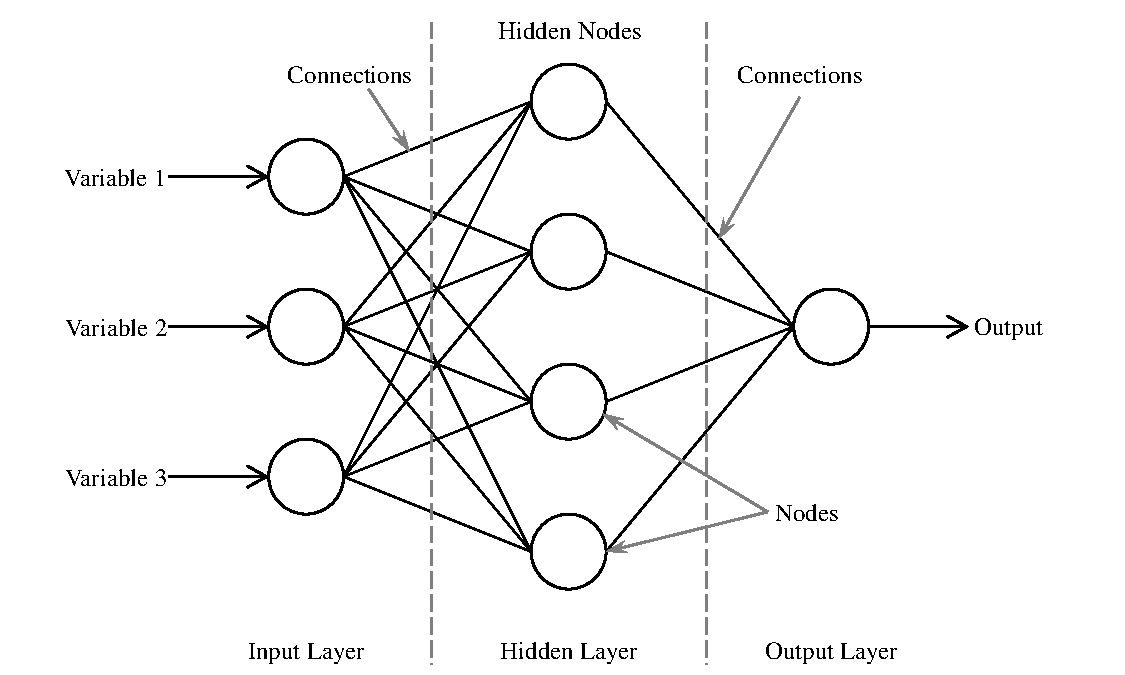
\includegraphics[width=0.95\linewidth]{figures/ANN_STRUCT.pdf} 
	\caption{An example of a generic Feed-Forward ANN structure.}
	\label{fig:ANN_STRUCT}
\end{figure}

Each of the models developed in this study were created using the Feed Forward type ANN, which is a unique algorithm used in machine learning that performs computations in a manner analogous to that of the human brain. This type of network requires sets of input data that are processed through a series of nodes and connections to ultimately produce an output, or an array of outputs, based on patterns recognized within the data set during training. A typical Feed-Forward ANN structure is presented in Fig. \ref{fig:ANN_STRUCT}. In this example, one sees that variable data is fed into the nodes located in the input layer. Data at the input nodes is then processed through the series of multiple connections present between nodes in the input layer and nodes in the hidden layer, each connection having its own associated weight. The combination of input data and weighted connection results in the data that is used as input at the hidden nodes. The data that has been fed into the hidden nodes is then processed through a second set of connections between the hidden layer and output layer in a likewise manner. This second set of combinations between data and weighted connections results in the data reported at the output node. It is important to note that during the development of the models presented in this study, the input data was first normalized using quantities that were based on the maximum and minimum values for each particular input variable. As such, the quantity reported to the output node must be expressed in real physical units by undoing the normalization that took place prior to the input layer using normalizing values that were also based on the maximum and minimum values of the recorded output in the training data set.

Each model network was developed using the following four step procedure. The first step was to choose what input variables and output information was desired. It is during this phase that the larger database of information constructed as described in Sec. \ref{sec:DBconstruct} above was mined for data presumed to be the most useful in producing an efficient model that could accurately predict boat-traffic. It is also during this step that the selected data must be separated into subsets for the purposes of training, testing, and validation, in an appropriate manner. Training sets often used approximately 50 \% of the given data sets, including at least one set that is representative of each maximum and minimum value of all selected inputs. This ensures that the model is trained on the full range of input data. The remaining data sets were divided between the testing and validation sets as evenly as possible. The second phase of development involved the initial training and testing of the different models for the purpose of determining the optimal amount of hidden nodes and iterations for training which would produce the most accurate predictions. This step will be explained further in Sec. \ref{sec:TrainTest} below. During the third stage of the development process, the three best performing networks in regard to the average-squared-error (ASE\SB{norm}), mean-absolute-relative-error (MARE\SB{norm}), and coefficient of determination (R\SPSB{2}{norm}) quantities, calculated using normalized values of predicted boat traffic and recorded boat traffic, were selected and tested with the validation data set and then re-trained on all data sets for the number of iterations found in step 2 in order to increase the accuracy of the final models, as models trained on larger data sets often display better accuracy measurement \cite{yasarer2012development}. Finally, the same error and accuracy measures stated in stage three of model development are compared between the final three models for the validation sets and the all data training sets, and the best performing model was selected. Actual comparisons for individual models are shown and discussed in Sec. \ref{sec:ComSel} below.

\subsection{Initial Training Process and Model Selection} \label{sec:TrainTest}

When the input data sets have been appropriately separated into training sets, testing sets, and validation sets, the network moves to the training phase. In this phase, normalizing factors are calculated based on the maximum and minimum values of each input, and all data is normalized as:

\begin{align}
\text{Y\SB{minANN}} &= \frac{P \cdot Y_{max} - \left(1 - P\right) \cdot Y_{min}}{2P-1}
\label{eq:YminANN}\\[0.5cm]
\text{Y\SB{maxANN}} &= \frac{Y_{max}-P\cdot Y_{minANN}}{1-P}
\label{eq:YmaxANN}\\[0.5cm]
\text{Input\SB{i,norm}} &= \frac{Input_{i} - Y_{minANN}}{Y_{maxANN}- Y_{minANN}}
\label{eq:NormInp}
\end{align}

Where Y\SB{minANN} is the lower bound of the considered domain of a given Input\SB{i}, Y\SB{maxANN} is the upper bound, Y\SB{min} is the minimum value of an Input\SB{i}, Y\SB{max} is the maximum value of an Input\SB{i}, P is a developer defined weighting factor between 0 and 0.5 (here considered as 0.2 for all input, and 0.1 for all output), and Input\SB{i, norm} is the final normalized input data to be introduced to the model.

At this point, the network begins its first training iteration. Normalized input data is fed into the input layer. Initial connection weights between the input layer and the hidden layer must be defined by the developer. This allows that the data in the input layer may be passed along to the hidden layer by summing the products of all normalized inputs and their connection weights (CW\SB{ij}) to a given hidden node as well as any Bias weight (Bias\SB{j}) assigned to the same hidden node (Equ. \ref{eq:NET}). The value of this summation of products and Bias is then passed as an argument to the logistic function (Equ.\ref{eq:logist}), the outcome of which defines the value of the corresponding hidden node (HN\SB{j}).
 
\begin{align}
\text{Net\SB{j}} &= \sum\limits_{i=1}^{N}\left(Input_{i,norm}\cdot CW_{ij}\right) + Bias_{j}
\label{eq:NET}\\[0.5cm]
\text{HN\SB{j}} &= \frac{1}{1+e^{-Net\SB{j}}}
\label{eq:logist}
\end{align}

The same method is then employed to transfer all data in the hidden layer to the output layer. The value of the output node (Y\SPSB{P}{norm}) is the result of the logistic function using the summation of the products of values at the hidden nodes and corresponding connection weights (CW\SB{j,Out}) between the hidden nodes and the output node in addition to any assigned Bias weight (Bias\SB{Out}) for the output node (Equ. \ref{eq:NETOUT}, Equ. \ref{eq:YP}).

\begin{align}
\text{Net\SB{Out}} &= \sum\limits_{j=1}^{N}\left(HN_{j}\cdot CW_{j,Out}\right) + Bias_{Out}
\label{eq:NETOUT}\\[0.5cm]
\text{Y\SPSB{P}{norm}} &= \frac{1}{1+e^{-Net\SB{Out}}}
\label{eq:YP}
\end{align}

This value is then re-dimensionalized so that the accompanying error may be recorded by taking the difference between the actual amount of boat traffic record and the prediction made by the network. This error quantity is then normalized and used in the back-propagation algorithm to adjust each of the connection weights and Bias weights present in the network accordingly. This process is repeated for each data set designated for training. Once every training data set has been processed through the network, and every accompanying error has been back-propagated to tune the network, a single iteration is considered complete.

In this study, initial training for all models was performed for 20,000 iterations with the beginning number of hidden nodes ranging from 5 to 15. Every 100\SP{th} iteration, the previously mentioned normalized error quantities (ASE\SB{norm}, MARE\SB{norm}, R\SPSB{2}{norm}) were measured for both the training set and the testing set, and the quantities were recorded for the purposes of comparison. This allowed the developer to note at what point the network performance was most accurate even while training over a large spectrum. It is important to note that when running the testing set, the error was not back-propagated into the network. At the conclusion of the 20,000\SP{th} iteration, a new hidden node would be introduced into the network until the number of hidden nodes reached 15. Upon reaching 15 hidden nodes, the network would run 20,000 more iterations and cease training.

Development would then enter the third and fourth stages, as described above, wherein all reported errors would be compared in order to located the best performing networks. Networks were then re-trained and tested on the validation data set. The best performing network of the validation set would be selected to be one of the final models presented in Table \ref{tab:ModStruct} below.

\begin{table}[h!]
	\centering
	\caption{Description of model structures.}
	\begin{tabular}{|l|c|c|c|c|}
		\hline
		\textbf{Models} & \textbf{Inputs} & \textbf{Hidden Nodes} & \textbf{Outputs} & \textbf{Prediction Type}\\\hline
		Model 1 & 24 & 15 & 1 & Daily\\\hline
		Model 2 & 16 & 15 & 1 & Daily\\\hline
		Model 3 & 19 & 15 & 1 & Daily\\\hline
		Model 4 & 21 & 15 & 1 & Daily\\\hline
		Model 5 & 8 & 10 & 1 & Daily\\\hline
		Model 6 & 55 & 15 & 1 & Daily\\\hline
		Model 7 & 28 & 10 & 1 & Daily\\\hline
		Model 8 & 13 & 9 & 1 & Hourly\\\hline
	\end{tabular}
	\label{tab:ModStruct}
	
\end{table}


\subsection{Model Comparison} \label{sec:ComSel}

Once training, testing, and validation are finalized, the networks selected to be the eight final models were then trained on all data and compared in order to assert what configuration led to the most accurate and most reasonable model for the purpose. 
Presented in Fig. \ref{fig:MOD1} through Fig. \ref{fig:MOD8} are the outcomes of plotting the desired target value against the final prediction produced by the models after being trained on all data, and Table \ref{tab:ModComp} presents the error resulting from this final training in normalized form.

 Fig. \ref{fig:ERRORS} shows an array of dimensionalized error quantities that will also be discussed in the comparisons to follow. The quantities reported in Fig. \ref{fig:ERRORS} were calculated using the following equations:


\begin{align}
\text{ASE} &= \frac{\sum\limits_{i=1}^{N}\sum\limits_{j=1}^{n}\left(Y_{ij}^{P}-Y_{ij}^{O}\right)^2}{N \cdot n}
\label{eq:ASE}\\[0.5cm]
%
\text{R\SP{2}} &=1 - \frac{\sum\limits_{i=1}^{N}\sum\limits_{j=1}^{n}\left(Y_{ij}^{O}-Y_{ij}^{P}\right)^2}{\sum\limits_{i=1}^{N}\sum\limits_{j=1}^{n}\left(Y_{ij}^{O}-\overline{Y_{i}^{O}}\right)^2}
\label{eq:RSQ}\\[0.5cm]
%
\text{MARE} &= \frac{\sum\limits_{i=1}^{N}\sum\limits_{j=1}^{n}\left(\frac{\mid Y_{ij}^{P}-Y_{ij}^{O} \mid}{Y_{ij}^{O}}\right) \cdot 100}{N \cdot n}
\label{eq:MARE}\\[0.5cm]
%
\text{RMSE} &= \sqrt{\frac{\sum\limits_{i=1}^{N}\sum\limits_{j=1}^{n}\left(Y_{ij}^{P}-Y_{ij}^{O}\right)^2}{N \cdot n}}
\label{eq:RMS}\\[0.5cm]
%
\text{MAE} &= \frac{\sum\limits_{i=1}^{N}\sum\limits_{j=1}^{n}\left(\mid Y_{ij}^{P}-Y_{ij}^{O} \mid\right)}{N \cdot n}
\label{eq:MAE}
\end{align}

Wherein $Y_{ij}^{P}$ is the predicted outcome, $Y_{ij}^{O}$ is the target outcome, $N$ is the number of data sets included in training the model, $n$ is the number of outputs of the model, and $\overline{Y_{i}^{O}}$ is the arithmetic mean of the target outcomes. It is important to note that in preparing the comparisons, the results for Model 8 were integrated in order to produce daily boat traffic as well.

 
\begin{table}[h!]
	\centering
	\caption{Accuracy measures of developed models for comparison. \textit{Model 8 predicts hourly boat traffic and should not be compared directly to other models.}}
	\resizebox{\linewidth}{!}{
	\begin{tabular}{|c|c|c|c|c|c|c|c|c||c|}
		\hline
		\multicolumn{2}{|c|}{\textbf{Models}}  & Model 1  & Model 2  & Model 3  & Model 4  & Model 5  & Model 6 & Model 7  & Model 8 \\ \hline
		\multirow{3}{*}{\rotatebox[]{90}{Train}}   &  ASE\SB{norm}   & 0.001445 & 0.009466 & 0.00475  & 0.003278 & 0.038209 &    0    & 0.001696 & \textit{0.006302} \\
		&  MARE\SB{norm}  &  12.778  &  31.833  &  20.988  &  18.201  &  98.637  &  0.497  &  51.567  &  \textit{76.687}  \\
		& R\SPSB{2}{norm} & 0.97995  & 0.87513  & 0.93426  & 0.95766  & 0.42697  &    1    & 0.96446  & \textit{0.61769}  \\ \hline
		\multirow{3}{*}{\rotatebox[]{90}{Test}}   &  ASE\SB{norm}   & 0.001438 & 0.009615 & 0.004778 & 0.003256 & 0.101697 &    0    & 0.005166 & \textit{0.006302} \\
		&  MARE\SB{norm}  &  12.131  &  31.639  &  20.353  &  17.797  & 129.694  &  0.466  &  68.475  &  \textit{81.184}  \\
		& R\SPSB{2}{norm} & 0.98002  & 0.87272  & 0.93383  & 0.95784  & 0.00477  & 0.99999 & 0.86555  & \textit{0.59216}  \\ \hline
		\multirow{3}{*}{\rotatebox[]{90}{Validate}} &  ASE\SB{norm}   & 0.001494 & 0.009849 & 0.004882 & 0.003232 & 0.182049 &    0    & 0.009986 & \textit{0.007202} \\
		&  MARE\SB{norm}  &  12.335  &  31.884  &  20.76   &  17.792  & 210.396  &  0.497  &  68.717  &  \textit{84.026}  \\
		& R\SPSB{2}{norm} & 0.97927  & 0.86967  & 0.93251  & 0.95838  & 0.26476  & 0.99999 & 0.76545  & \textit{0.54269}  \\ \hline
	\end{tabular}
			}
	\label{tab:ModComp}
\end{table}

\subsubsection{Model 1}
The categorical inputs for model one included 5 inputs representing the month of the year during which counts were recorded, 7 inputs representing the day of the week on which counts were recorded, 1 input to represent whether the day on which counts took place was a holiday, 3 inputs representing weather conditions on the day of the counts, and 4 inputs representing the location of the boating events. The numerical input considered for this model consisted of precipitation data, temperature data, local water depth measured at the instant of a given count, and local river stage measured at the instant of a given count. This was the first model constructed and includes all the raw data that was acquired from the Connecticut River, without further consideration.This model also served as the baseline from which other models were created. 

Model one was trained on 19,432 data sets, treating each instant a passing vessel was recorded as a separate data set. It is the second best performing model in terms all 5 considered error quantities. However, this is likely due to the presence of a large amount of categorical input in contrast to the very small amount of numerical input. 

\subsubsection{Model 2}

Model 2 was created in response to the unexpected accuracy of predictions given by model 1. In order to analyze how dependent the model was on categorical input, 8 inputs were removed. These 8 consisted of the month of the year and the categorical weather conditions. It was deemed fitting to remove the month of the year input as the data set is only representative of 5 months of 1 year spanning roughly 1 season. This likely provided little insight for the network to learn from as compared to other categorical inputs such as the inputs regarding the day of the week, which were cycled through multiple times in various conditions. The categorical weather conditions were deemed potentially redundant as the model also includes numerical data for temperature and precipitation. 

This model was trained on the same number of data sets as model 1. Once fully trained, a stark decrease in performance was observed between model 1 and model 2. ASE increased by approximately 550\%, while the other measures were seen to be in excess of 200\% of corresponding quantities in model 1. In order to test what inputs were more influential in the decreased performance, models 3 and 4 were made in parallel.

\subsubsection{Model 3}

Model 3 re-introduced the categorical weather conditions to model 2. The model was trained on the same number of data sets as those preceding it. Upon completion of training, it was observed that the performance of this model was very similar to that of model 2 with negligible improvement. This observation verified the idea of categorical weather conditions being redundant within the model.

\subsubsection{Model 4}

Model 4 re-introduced the categorical inputs regarding month of the year to model 2 and was also trained on the same number of data sets as those preceding it. Once trained, a large improvement in performance was seen relative to the performance of model 2. This model's performance is not as accurate as model 1 but is reasonably comparable, showing that the categorical inputs regarding the month of the year had much more influence on the accuracy of network predictions than initially believed.
 
\subsubsection{Model 5}

Model 5 was also used as a reference. The only inputs utilized in this model were the 4 previously mentioned numerical inputs and the 4 categorical inputs representing location. As expected, this model performs poorly, ranking last in every accuracy measure considered in this study. Though it was trained on the same number of data sets as models 1, 2, 3, and 4, it suffers from a lack of variety in the data. Because of the restriction to 8 inputs and the short time span in which raw data was recorded, the network is not presented with any notable pattern between the given inputs and the desired predictions. 

This is due to the fact that the model is representative of a single, short reach of the Connecticut River and is restricted to a single season's measurements. Because of this, much of the input data appears similar as it is all relative to the same location. However, since there is a vast amount of difference in the boat traffic of different days, there is no discernible connection between the inputs and the output. This implies that there is significant importance in having some time factor present when predicting boat-traffic.

\subsubsection{Model 6}

Model 6 introduces an additional 31 categorical inputs. These are for the purpose of identifying the day of the month in which the counts take place. As there is such an overwhelming amount of categorical input in this model, based on what was observed in model 1, it was expected that this model would perform extremely well. This held true, as the model produces near perfect results. ASE for model 6 was calculated to be 0.006, R\SP{2} was shown to be 1, MARE was 0.276\%, RMSE was 0.079, and the MAE was 0.011. However, this model is a exemplary case of over training. Being trained on the same number of data sets as all other models, with 51 categorical inputs, the network has more than enough data to track a pattern and begin memorizing the desired output.

\subsubsection{Model 7}

Model 7 is a far more robust network. This model introduced the concept of memory to the network development. Rather than considering only the data corresponding to the day of the count, this model also includes data relating to the day prior. This was also the model that introduced the numerical representation of the weekday by utilizing the probabilistic weights described in Sec. \ref{sec:DBconstruct}, as well as the use of daily maximums and minimums for the values of the aforementioned numerical data considered in other models. This resulted in the final form of the data sets used in the construction of model 7 having 16 numerical inputs and 12 categorical inputs. This model was trained on only 416 data sets but produces results comparable to those of model 1, though it is worth noting that this model did not perform as well in the testing and validation phase of network development, as seen in Table \ref{tab:ModComp}.

\subsubsection{Model 8}

Model 8 was developed to explore the idea of predicting daily boat traffic by integrating predictions of hourly boat traffic. This model removed the consideration of memory from development, but still employs the use of the probabilistic weight as the sole time factor. The remaining 12 inputs are the same as those employed in model 1. Each data set is representative of a single hour during the time of recording, at various locations. This model was trained on 3,972 data sets and performs to the same level of adequacy as model 2 and model 3.

\section{Conclusion}

In order to predict daily boat traffic in a 32-km reach of the Connecticut River, models were created using the Feed-Forward Artificial Neural Network approach with the back-propogation-of-error algorithm. Of the 8 models produced in this study, statistical accuracy measures vary based on the type of data presented for training. However, as can be seen in Table \ref{tab:ModComp} and Fig. \ref{fig:MOD1} through Fig. \ref{fig:ERRORS}, results show promise. Model 1 and Model 7 were shown to be the best performing models developed in terms of reasonable and accurate results regarding the accuracy measures considered; the notable exception being Model 5 which was over trained on a large amount of categorical data. With a larger database representing the same data types compiled over a longer period of time, the performance of these models is only expected to improve. Future work will seek to incorporate a larger amount of data, varying geographical location in a single model, an indication of vessel type in order to developed a model that is not only accurate in prediction of boat traffic, but valid for use in a greater scope of locale and able to predict the assortment of different types of high-speed vessels.

%-----------



%\begin{enumerate}
%	\item Guess an initial depth at which to begin iterations, i.e. $h_o = 1$
%	\item Use Equ. \ref{eq:h02} to calculate the corresponding celerity $c_{tc}$
%	\item Use this $c_{tc}$ to solve Equ. \ref{eq:h01} for the corresponding downstream depth, $h_o$
%	\item If the two values of $h_o$ are sufficient close so as to presume acceptable accuracy in approximation, discontinue the iterative process. If not, begin again supposing the initial guess to be the final value of $h_o$ of the last iteration.
%\end{enumerate}


%\begin{figure}[h!]
%	\centering
%	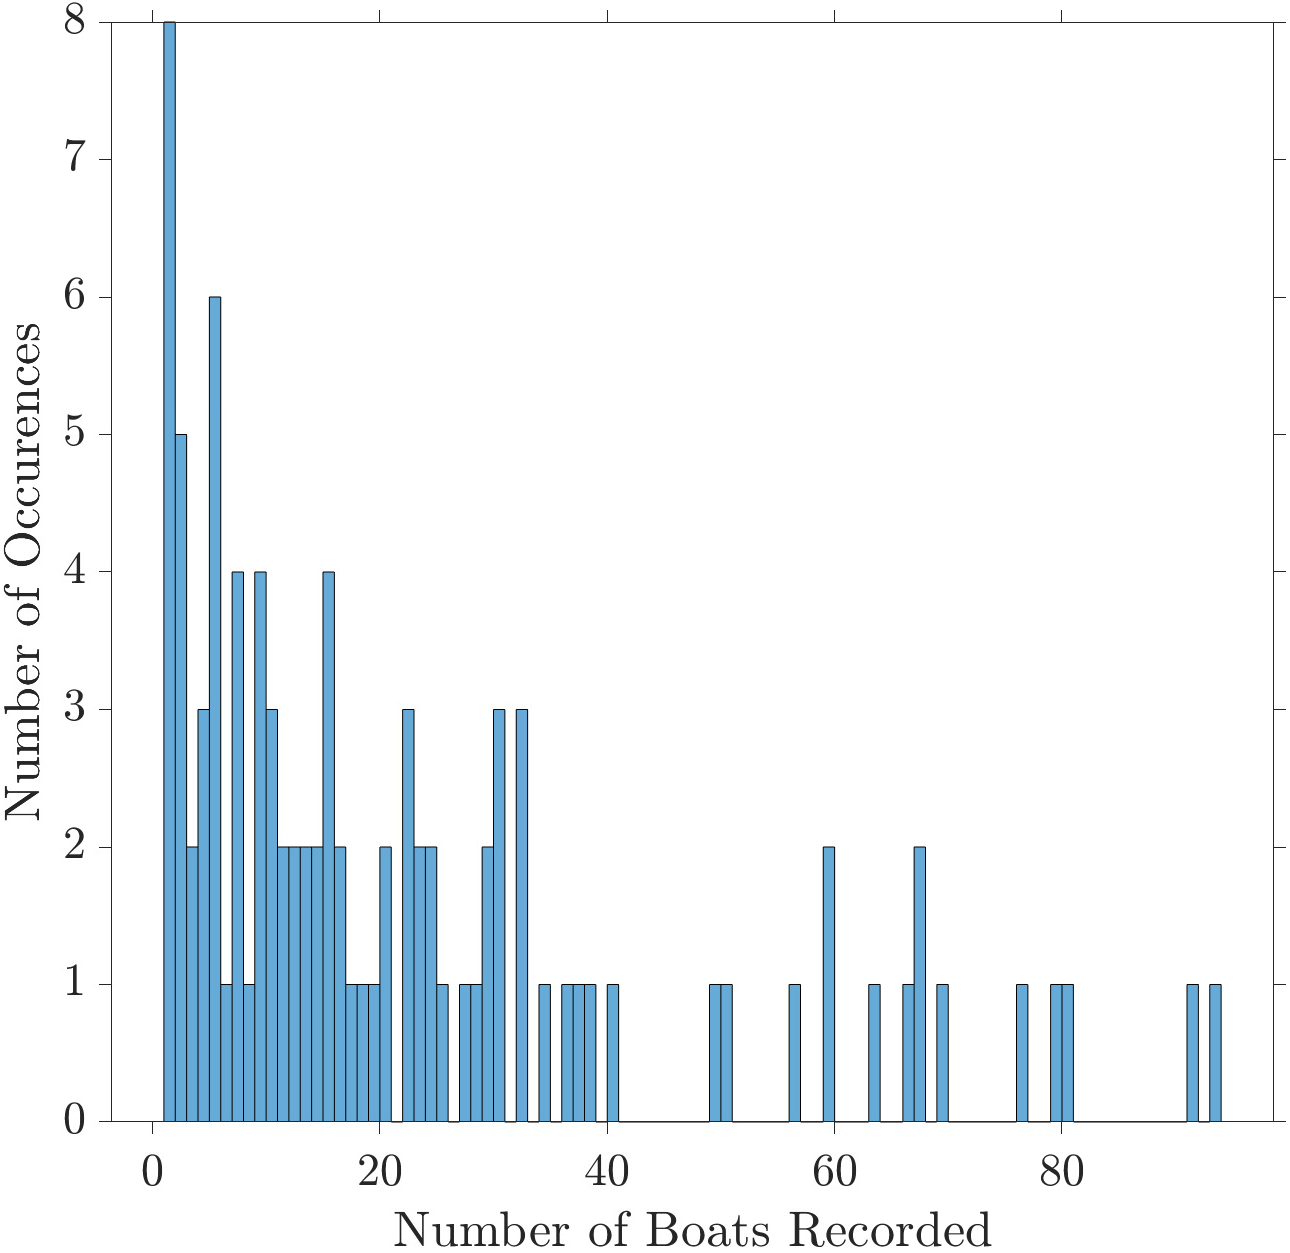
\includegraphics[width=0.49\linewidth]{figures/LOG1.pdf} 
%	\caption{Frame of dam break animation in a wetted channel with trajectories captured at time = 50 seconds.}
%	\label{fig:PosWave}
%\end{figure}
\newpage
\printbibliography
\newpage
\begin{figure}[h!]
	\centering
	\begin{subfigure}[t]{0.49\linewidth}
		\centering
		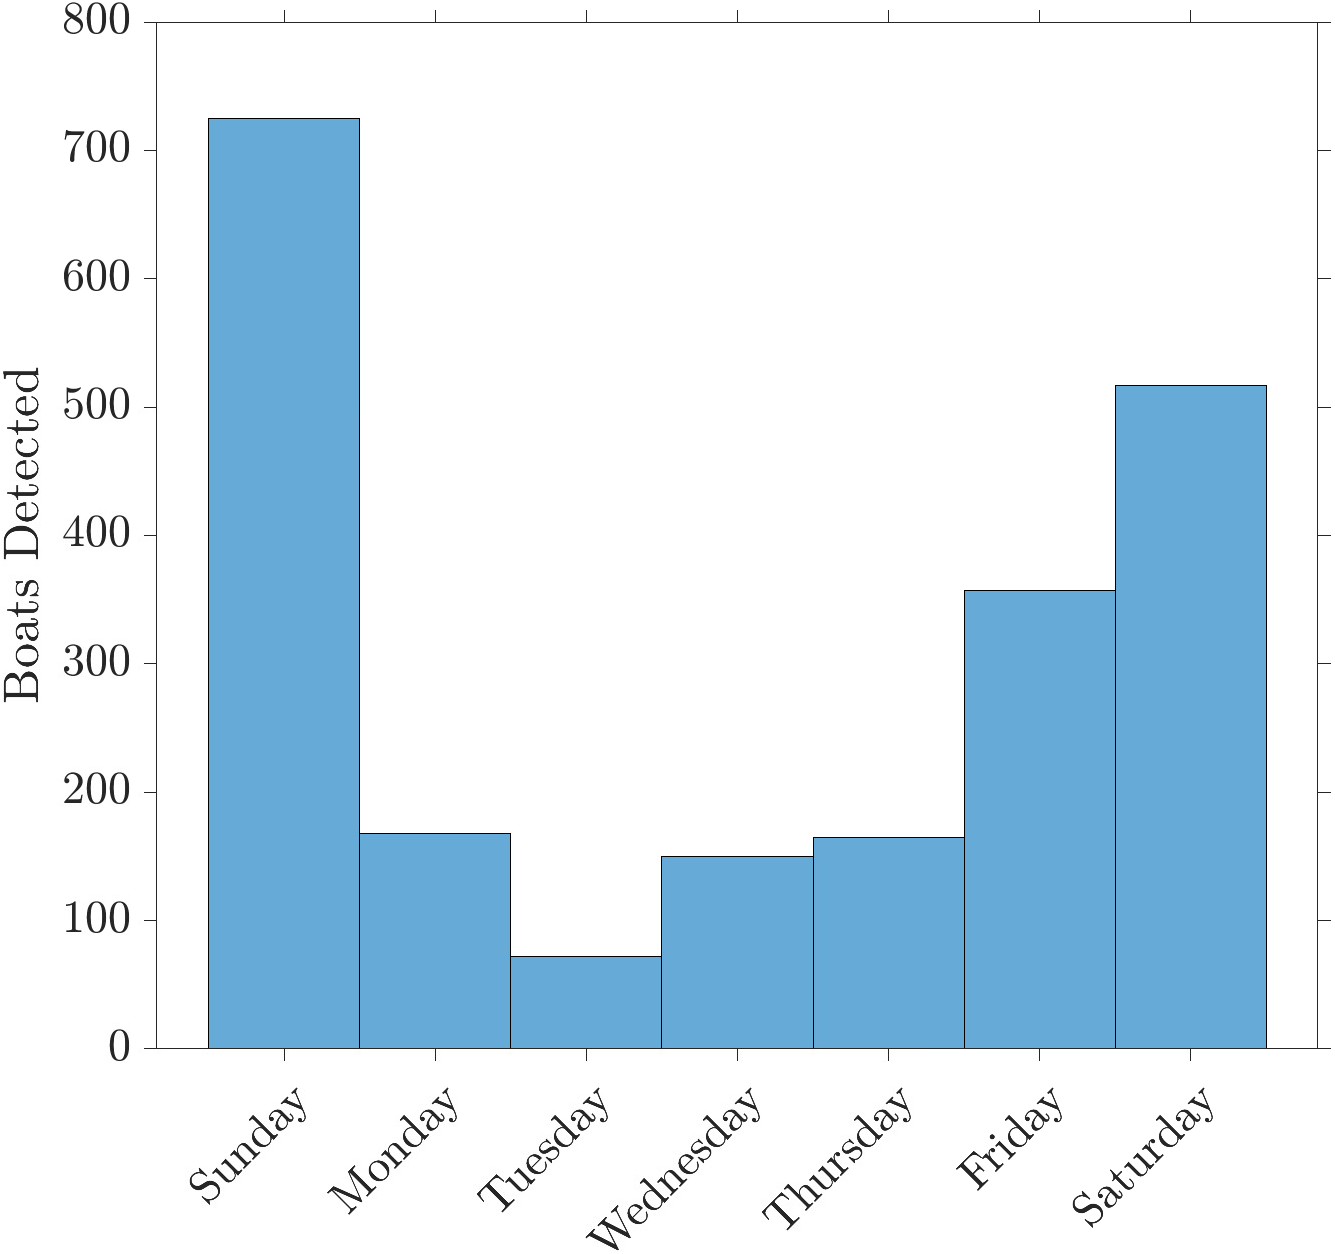
\includegraphics[width=\linewidth]{figures/WeekDayHist_LOG1.pdf}
		\caption{Wave Staff 1} 
		\label{fig:WeekL1}
	\end{subfigure}
	%
	\begin{subfigure}[t]{0.49\linewidth}
		\centering
		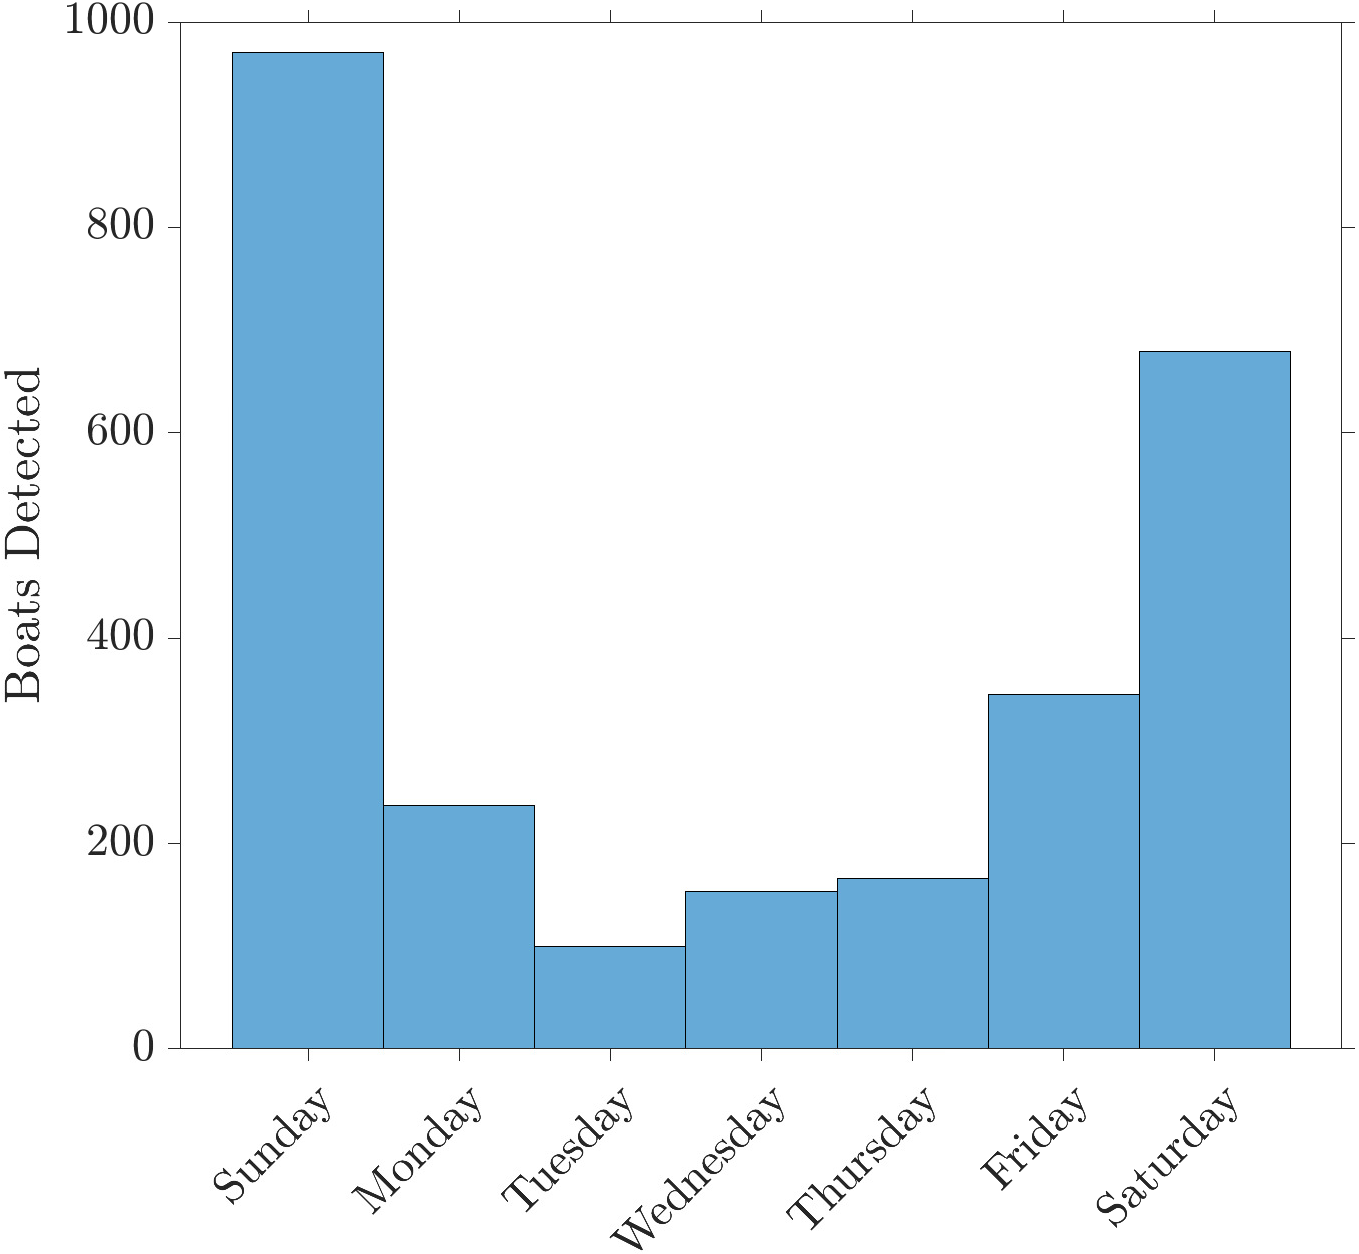
\includegraphics[width=\linewidth]{figures/WeekDayHist_LOG2.pdf}
		\caption{Wave Staff 2} 
		\label{fig:WeekL2}
	\end{subfigure}
	%
	\begin{subfigure}[t]{0.49\linewidth}
		\centering
		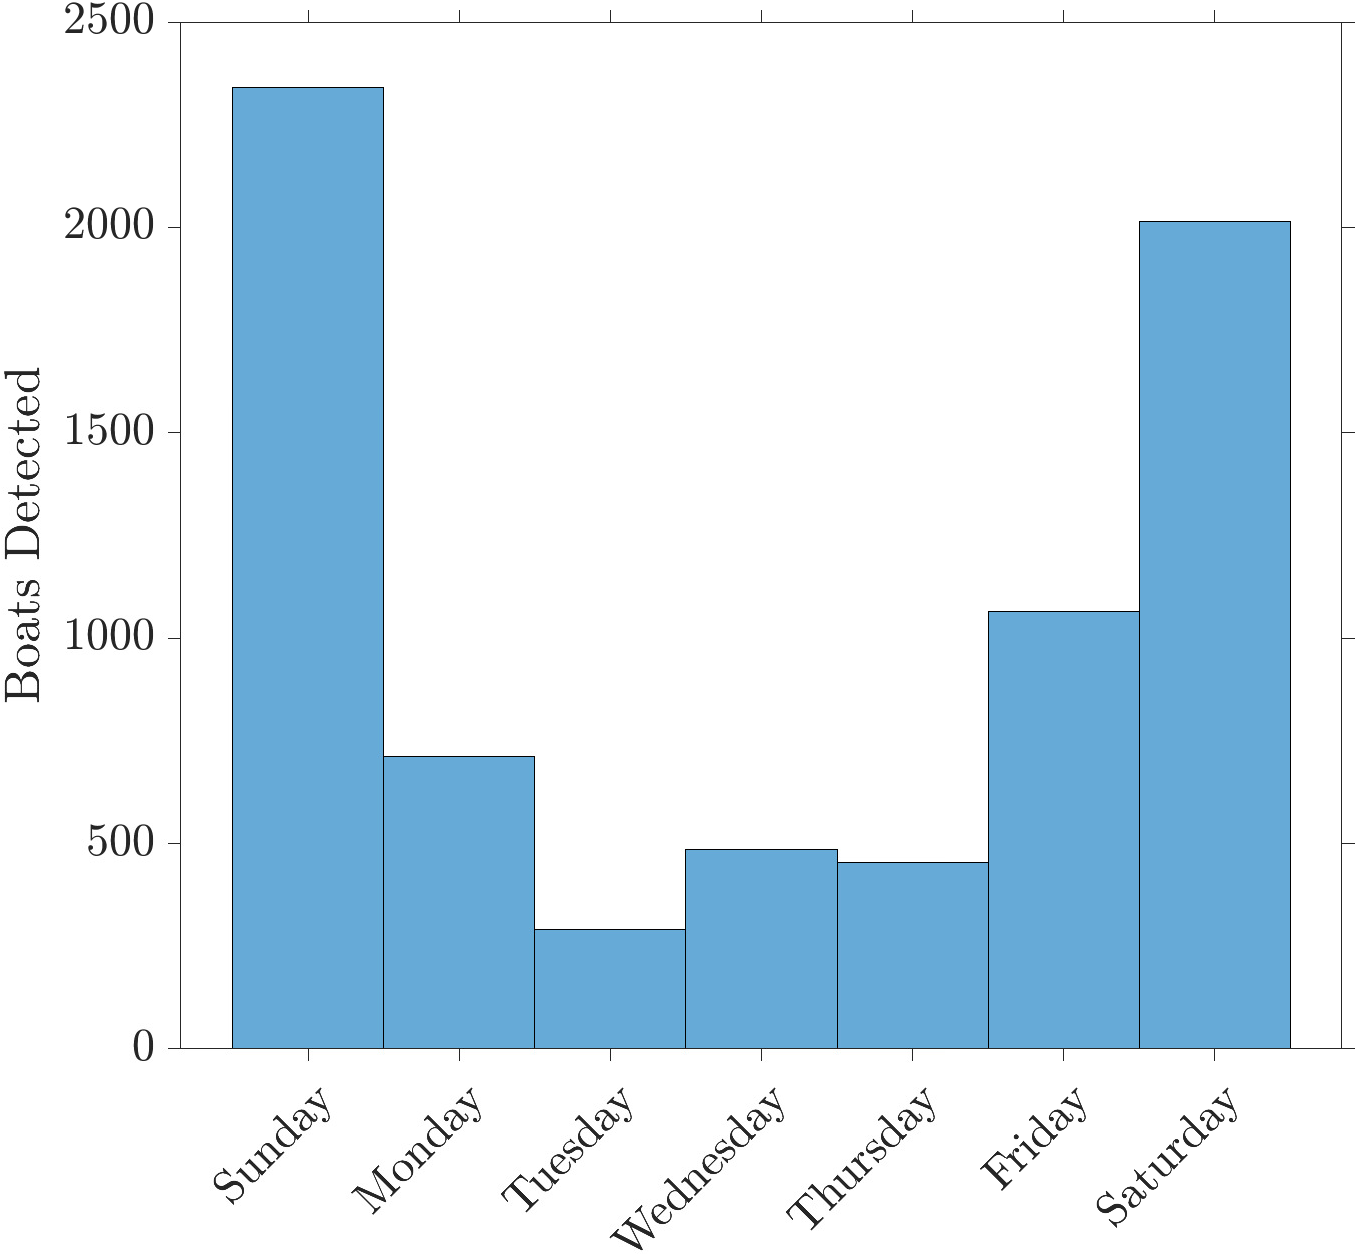
\includegraphics[width=\linewidth]{figures/WeekDayHist_LOG3.pdf}
		\caption{Wave Staff 3} 
		\label{fig:WeekL3}
	\end{subfigure}
	%
	\begin{subfigure}[t]{0.49\linewidth}
		\centering
		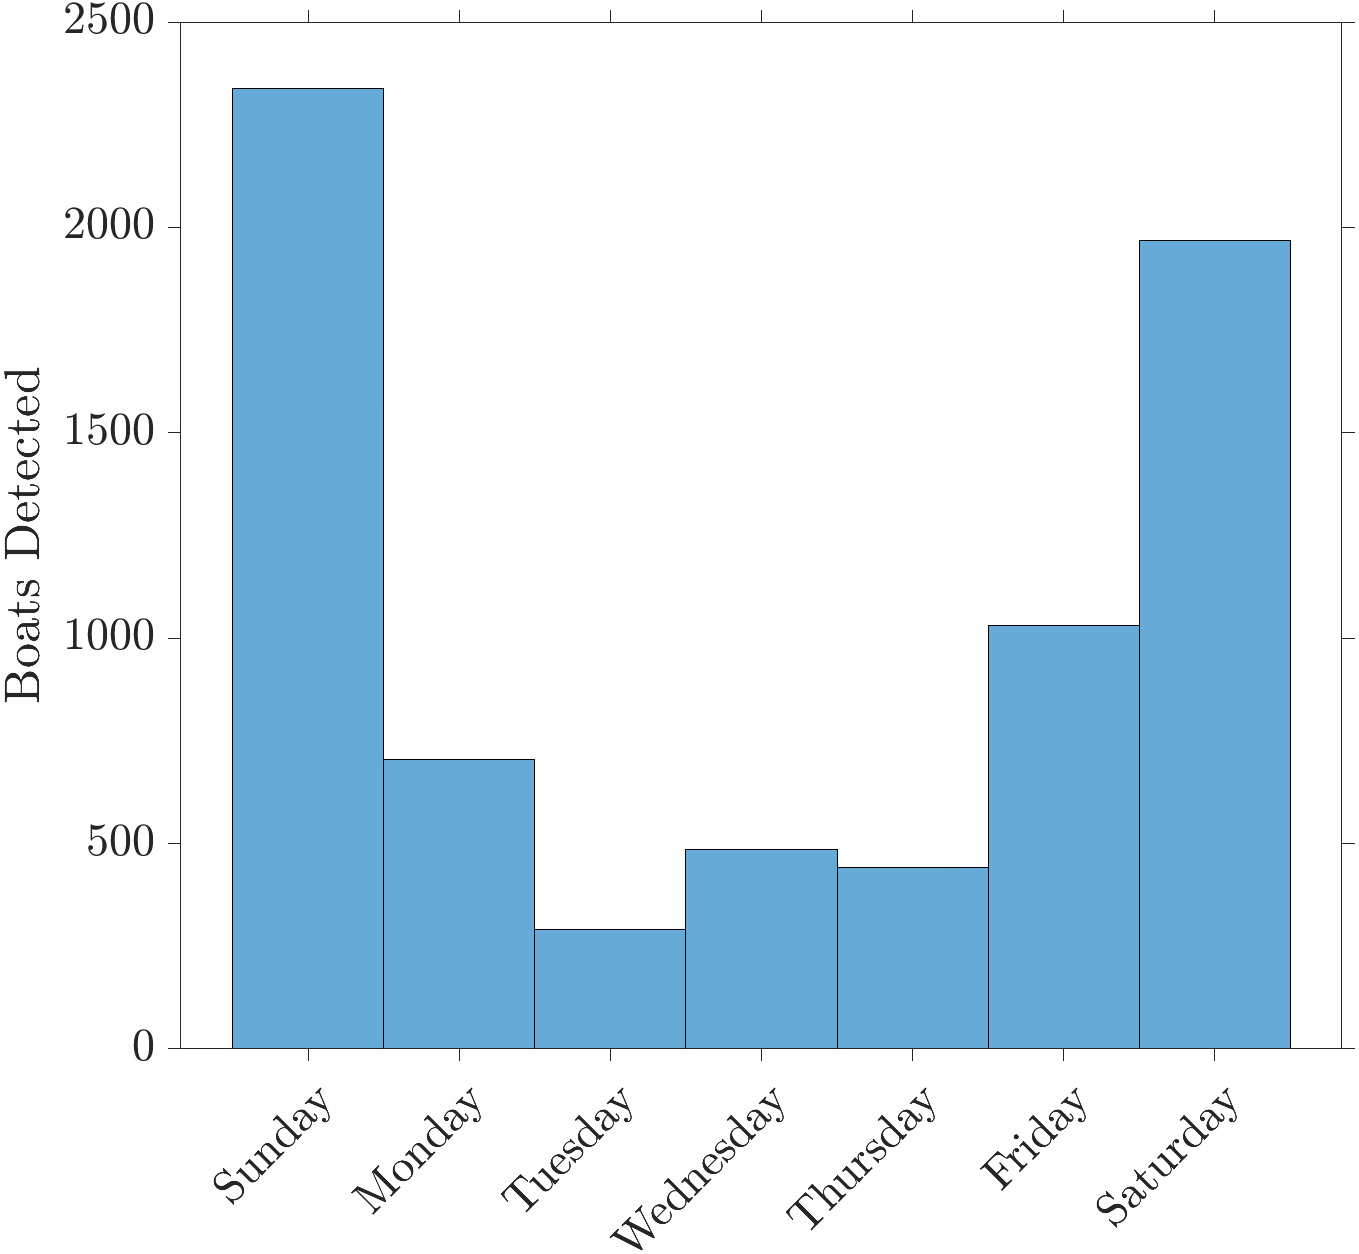
\includegraphics[width=\linewidth]{figures/WeekDayHist_LOG4.pdf}
		\caption{Wave Staff 4} 
		\label{fig:WeekL4}
	\end{subfigure}
	\caption{Histograms of boat traffic for given weekdays recorded at different location.}
	\label{fig:Weekdays}
\end{figure}

\begin{figure}[h!]
	\centering
	\begin{subfigure}[t]{0.49\linewidth}
		\centering
		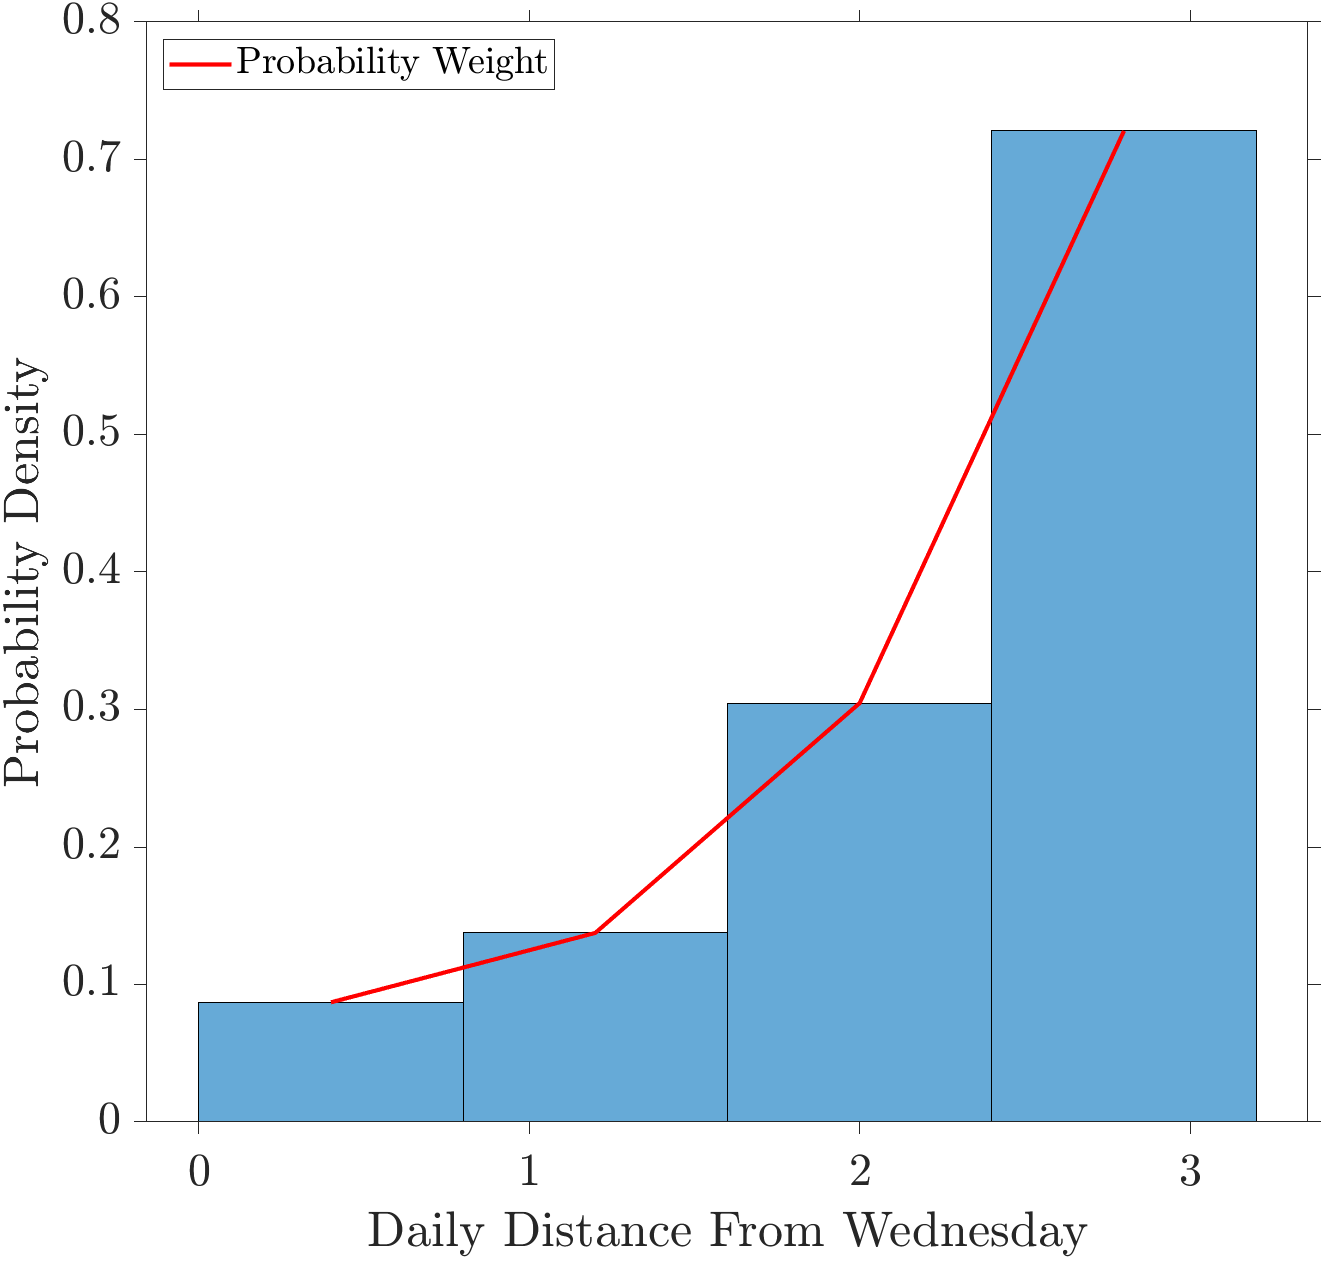
\includegraphics[width=\linewidth]{figures/PDF_LOG1.pdf}
		\caption{Wave Staff 1} 
		\label{fig:PDFL1}
	\end{subfigure}
	%
	\begin{subfigure}[t]{0.49\linewidth}
		\centering
		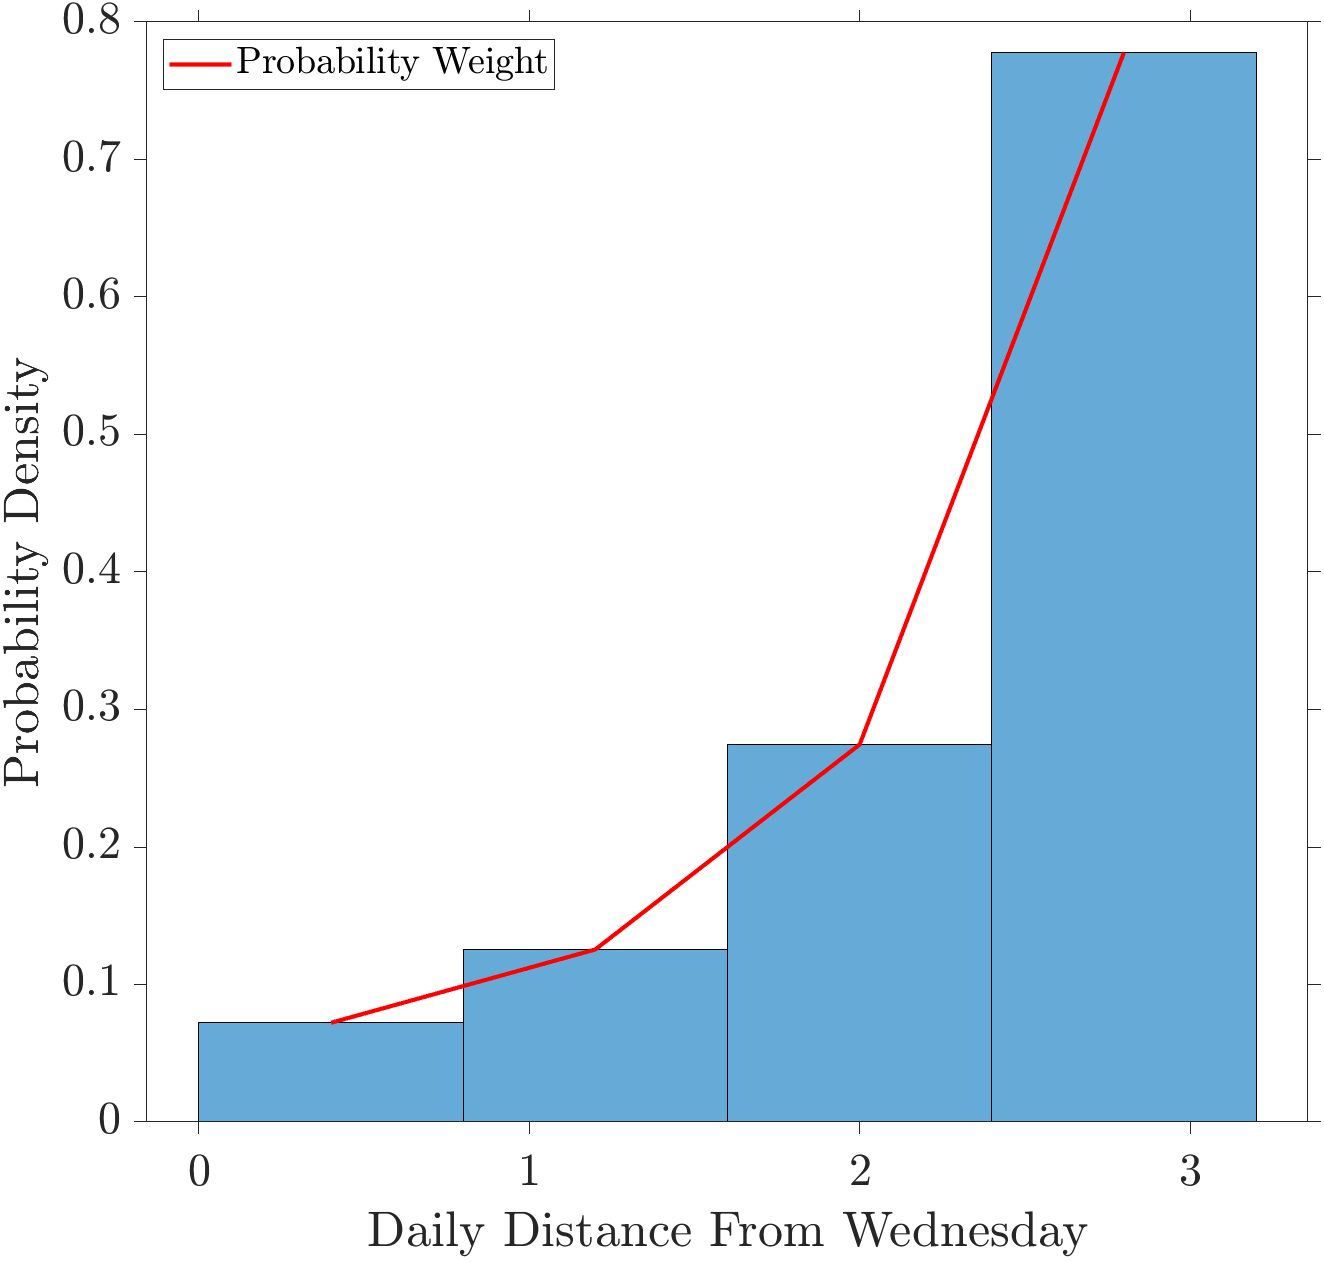
\includegraphics[width=\linewidth]{figures/PDF_LOG2.pdf}
		\caption{Wave Staff 2} 
		\label{fig:PDFL2}
	\end{subfigure}
	%
	\begin{subfigure}[t]{0.49\linewidth}
		\centering
		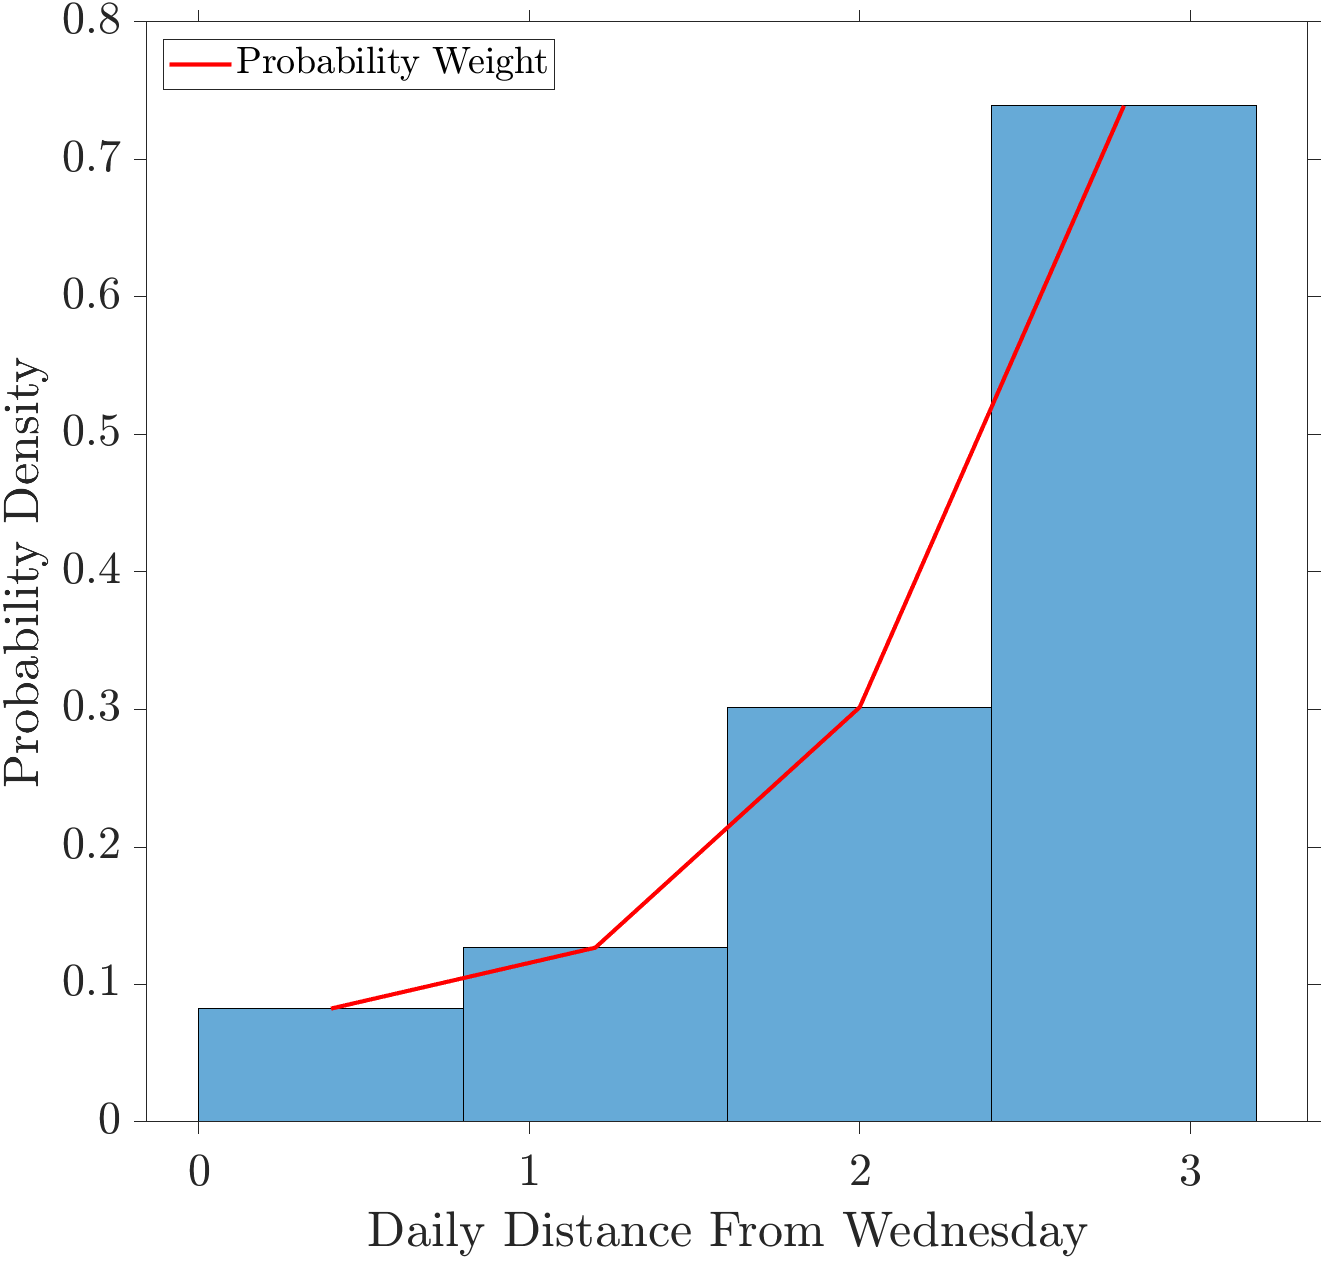
\includegraphics[width=\linewidth]{figures/PDF_LOG3.pdf}
		\caption{Wave Staff 3} 
		\label{fig:PDFL3}
	\end{subfigure}
	%
	\begin{subfigure}[t]{0.49\linewidth}
		\centering
		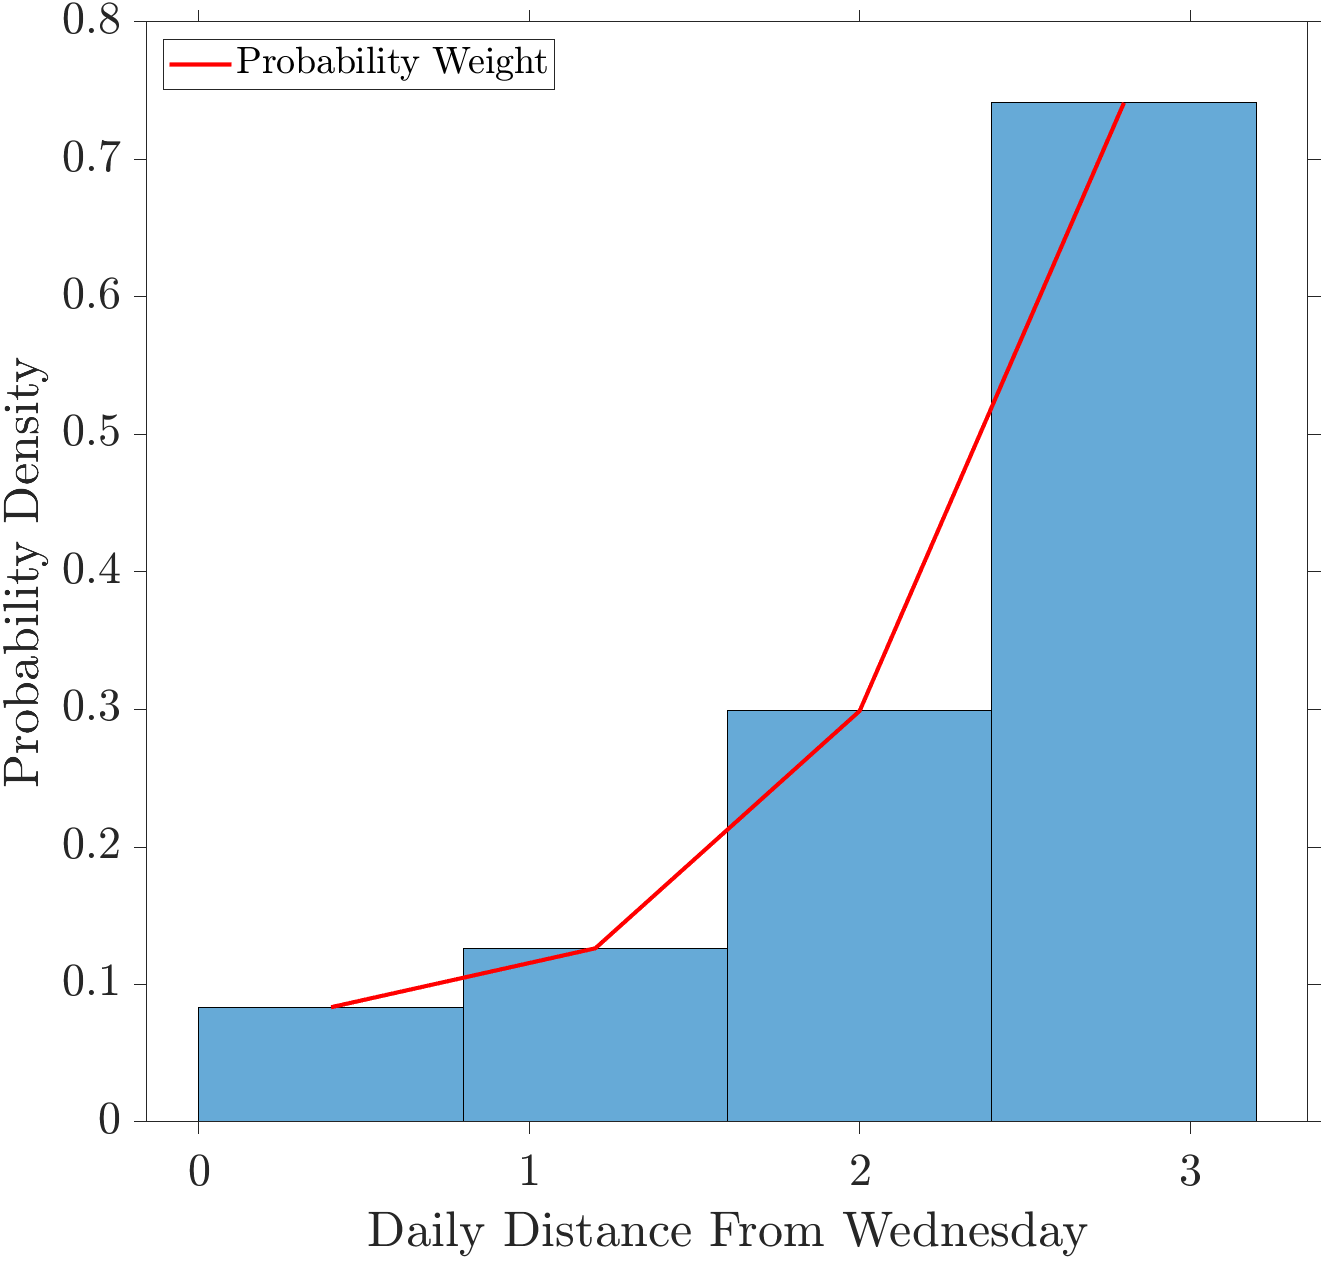
\includegraphics[width=\linewidth]{figures/PDF_LOG4.pdf}
		\caption{Wave Staff 4} 
		\label{fig:PDFL4}
	\end{subfigure}
	\caption{Normalized histogram represent the probability density function of boat traffic based on daily distance from Wednesday.}
	\label{fig:PDFs}
\end{figure}

\begin{figure}[h!]
	\centering
	\begin{subfigure}[t]{0.49\linewidth}
		\centering
		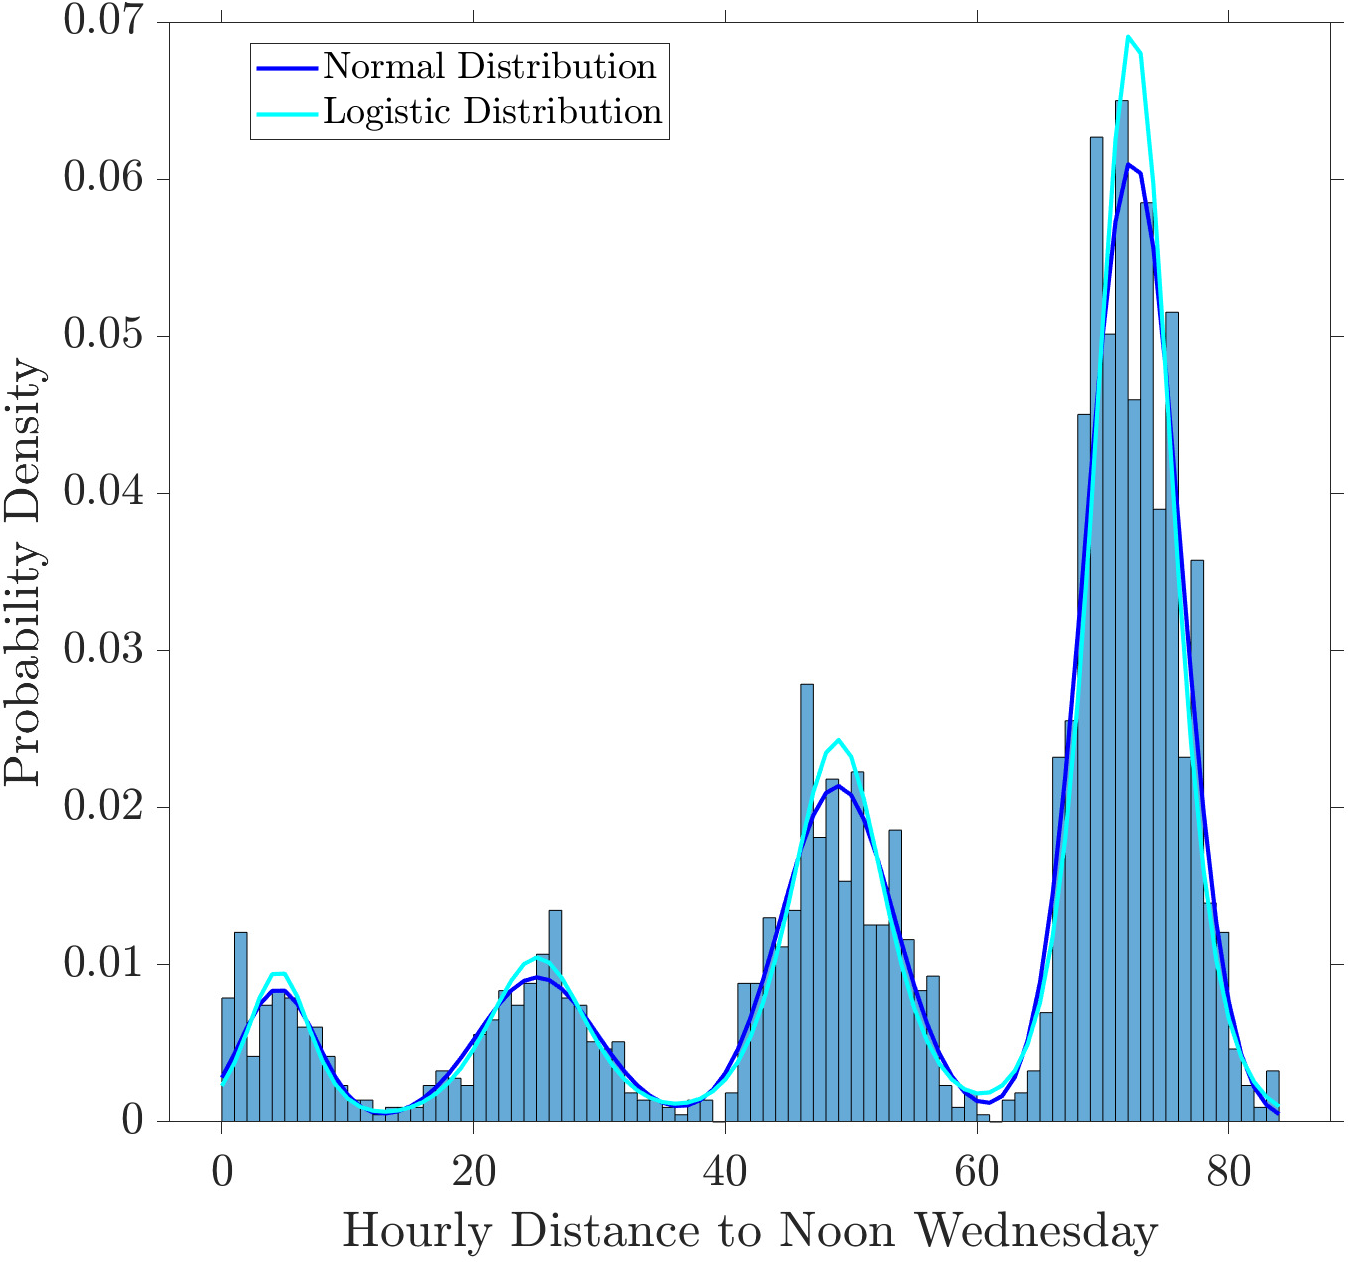
\includegraphics[width=\linewidth]{figures/HourPDF_LOG1.pdf}
		\caption{Wave Staff 1} 
		\label{fig:HourL1}
	\end{subfigure}
	%
	\begin{subfigure}[t]{0.49\linewidth}
		\centering
		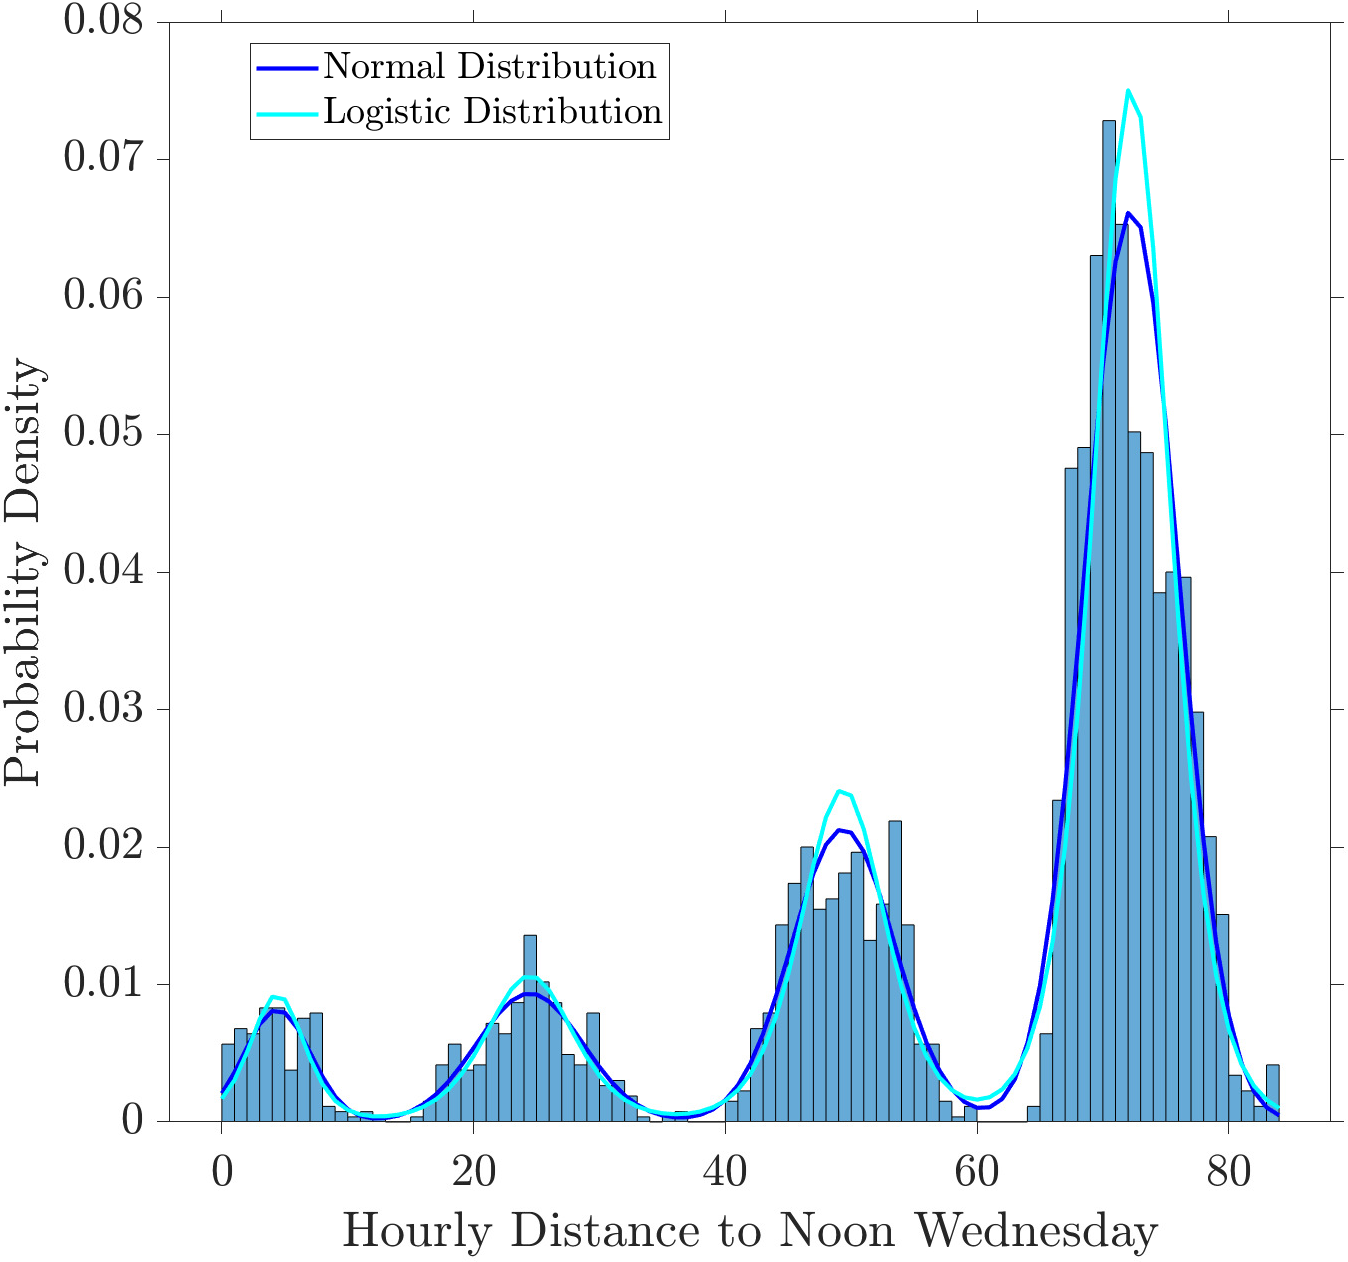
\includegraphics[width=\linewidth]{figures/HourPDF_LOG2.pdf}
		\caption{Wave Staff 2} 
		\label{fig:HourL2}
	\end{subfigure}
	%
	\begin{subfigure}[t]{0.49\linewidth}
		\centering
		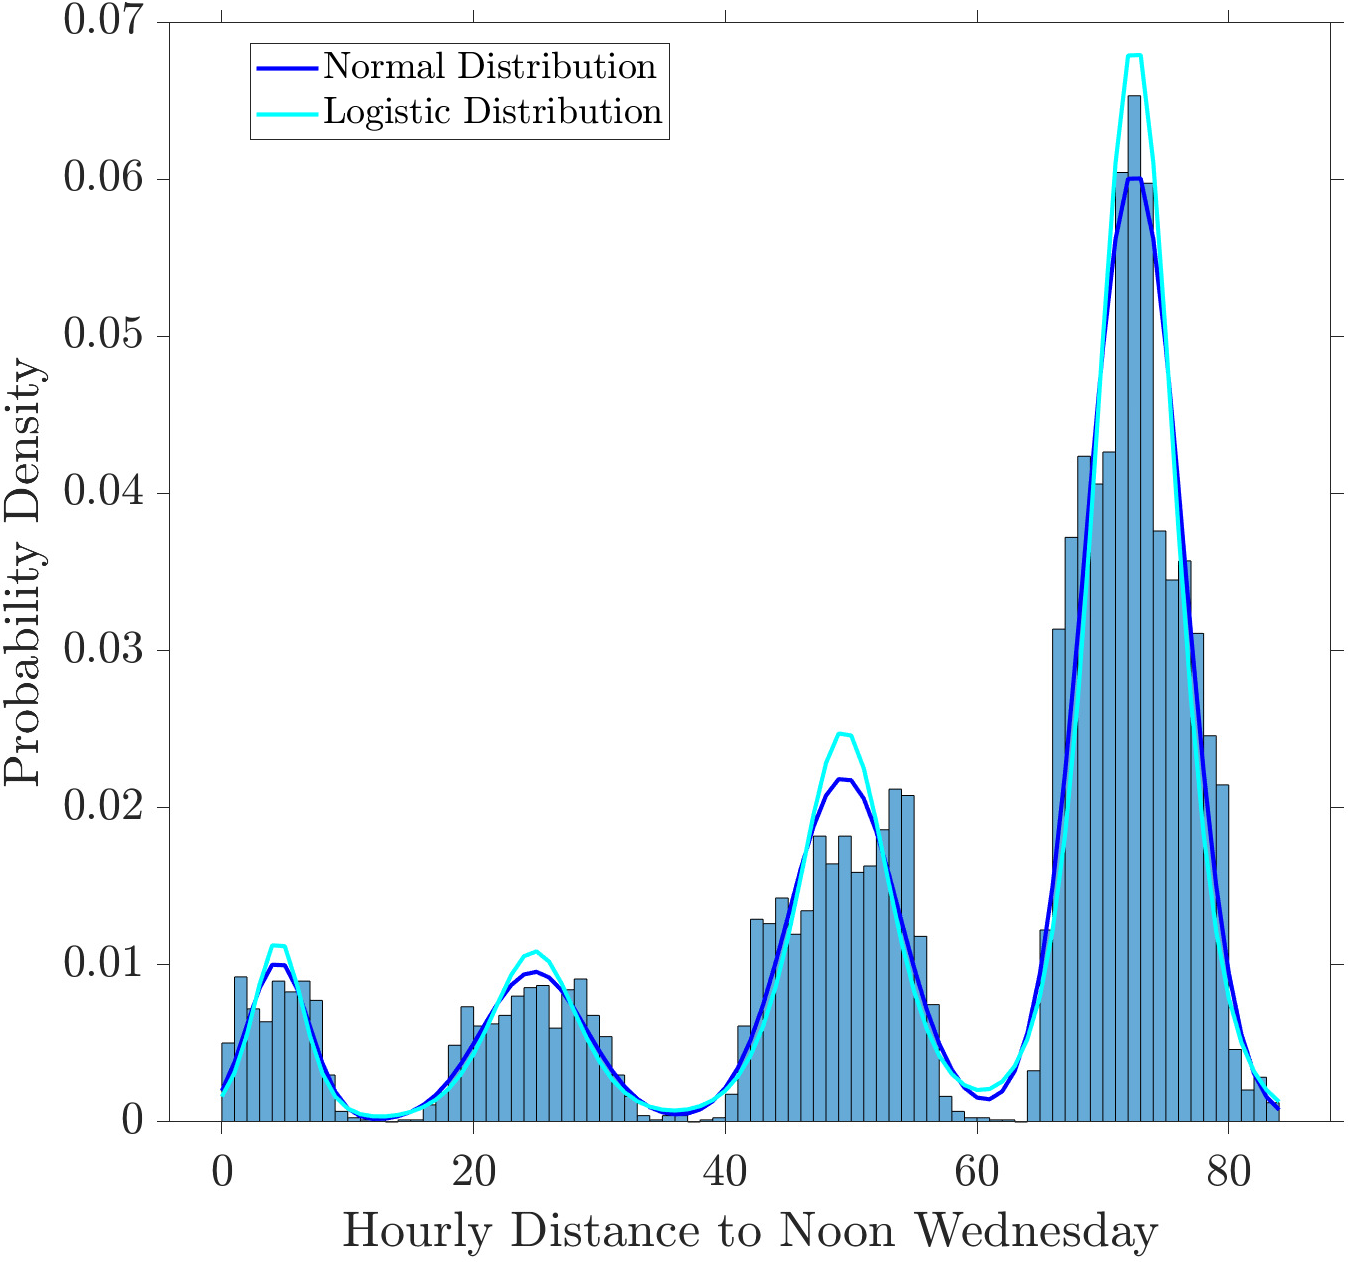
\includegraphics[width=\linewidth]{figures/HourPDF_LOG3.pdf}
		\caption{Wave Staff 3} 
		\label{fig:HourL3}
	\end{subfigure}
	%
	\begin{subfigure}[t]{0.49\linewidth}
		\centering
		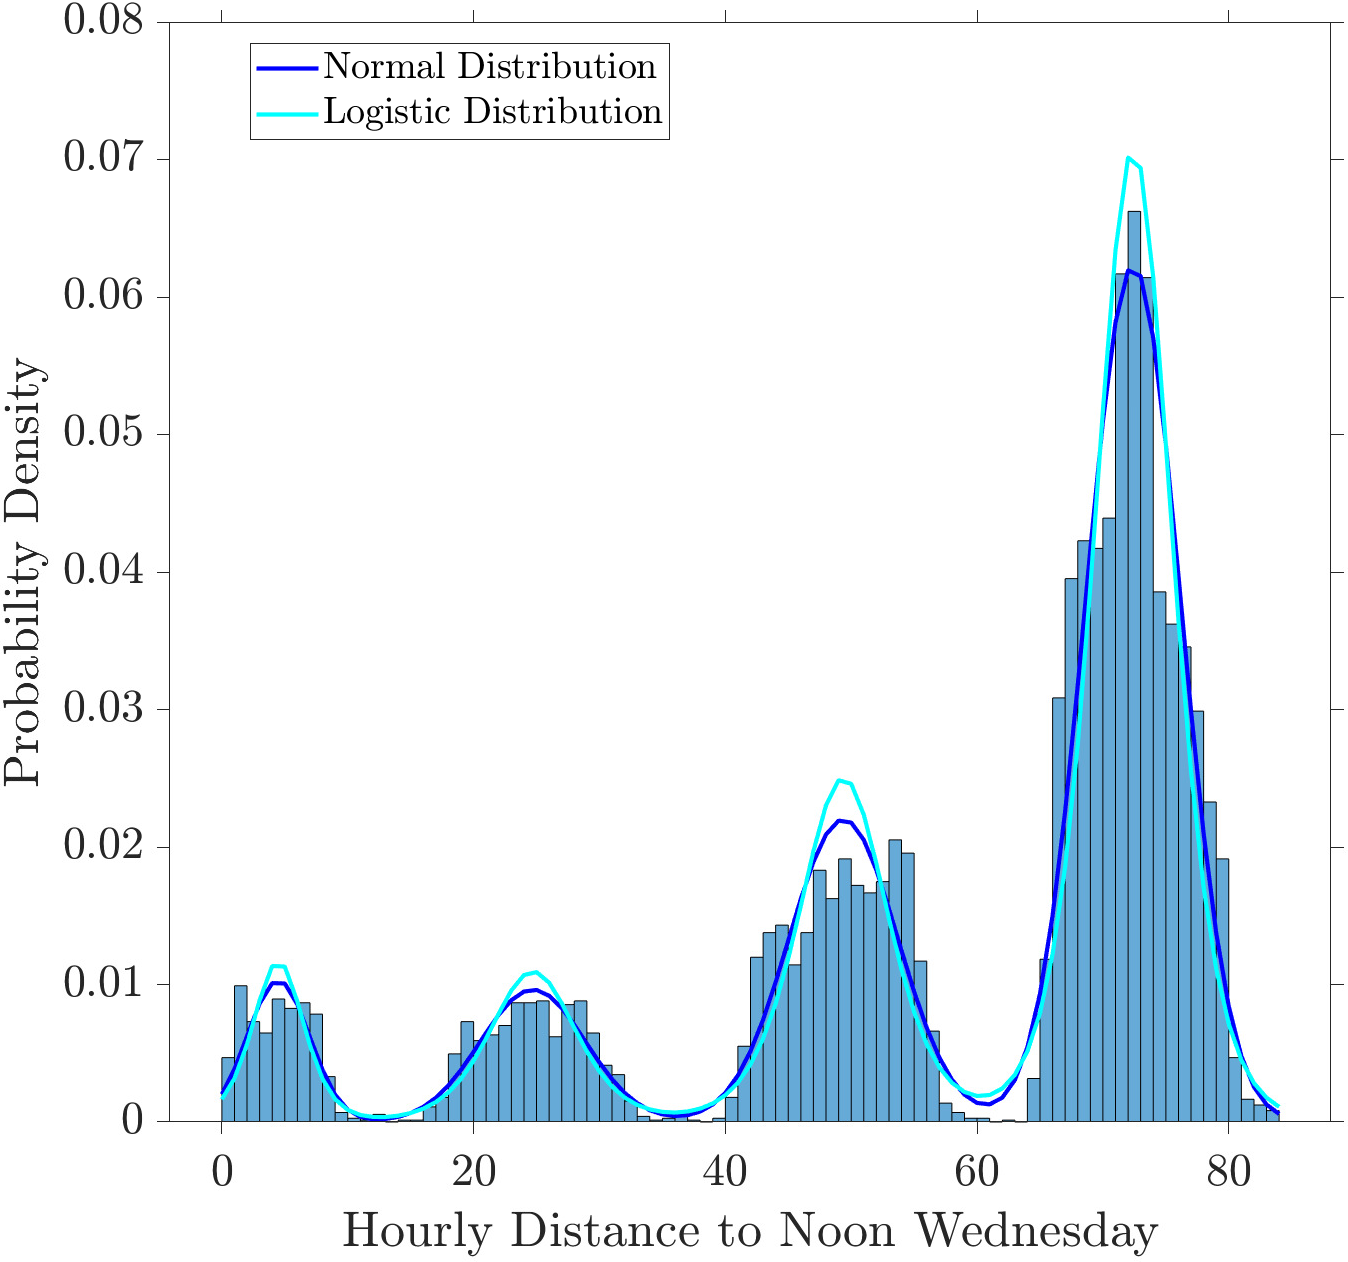
\includegraphics[width=\linewidth]{figures/HourPDF_LOG4.pdf}
		\caption{Wave Staff 4} 
		\label{fig:HourL4}
	\end{subfigure}
	\caption{Normalized histogram represent the probability density function of boat traffic based on hourly distance from noon on Wednesday.}
	\label{fig:Hourly}
\end{figure}

	\begin{figure}
	\centering
	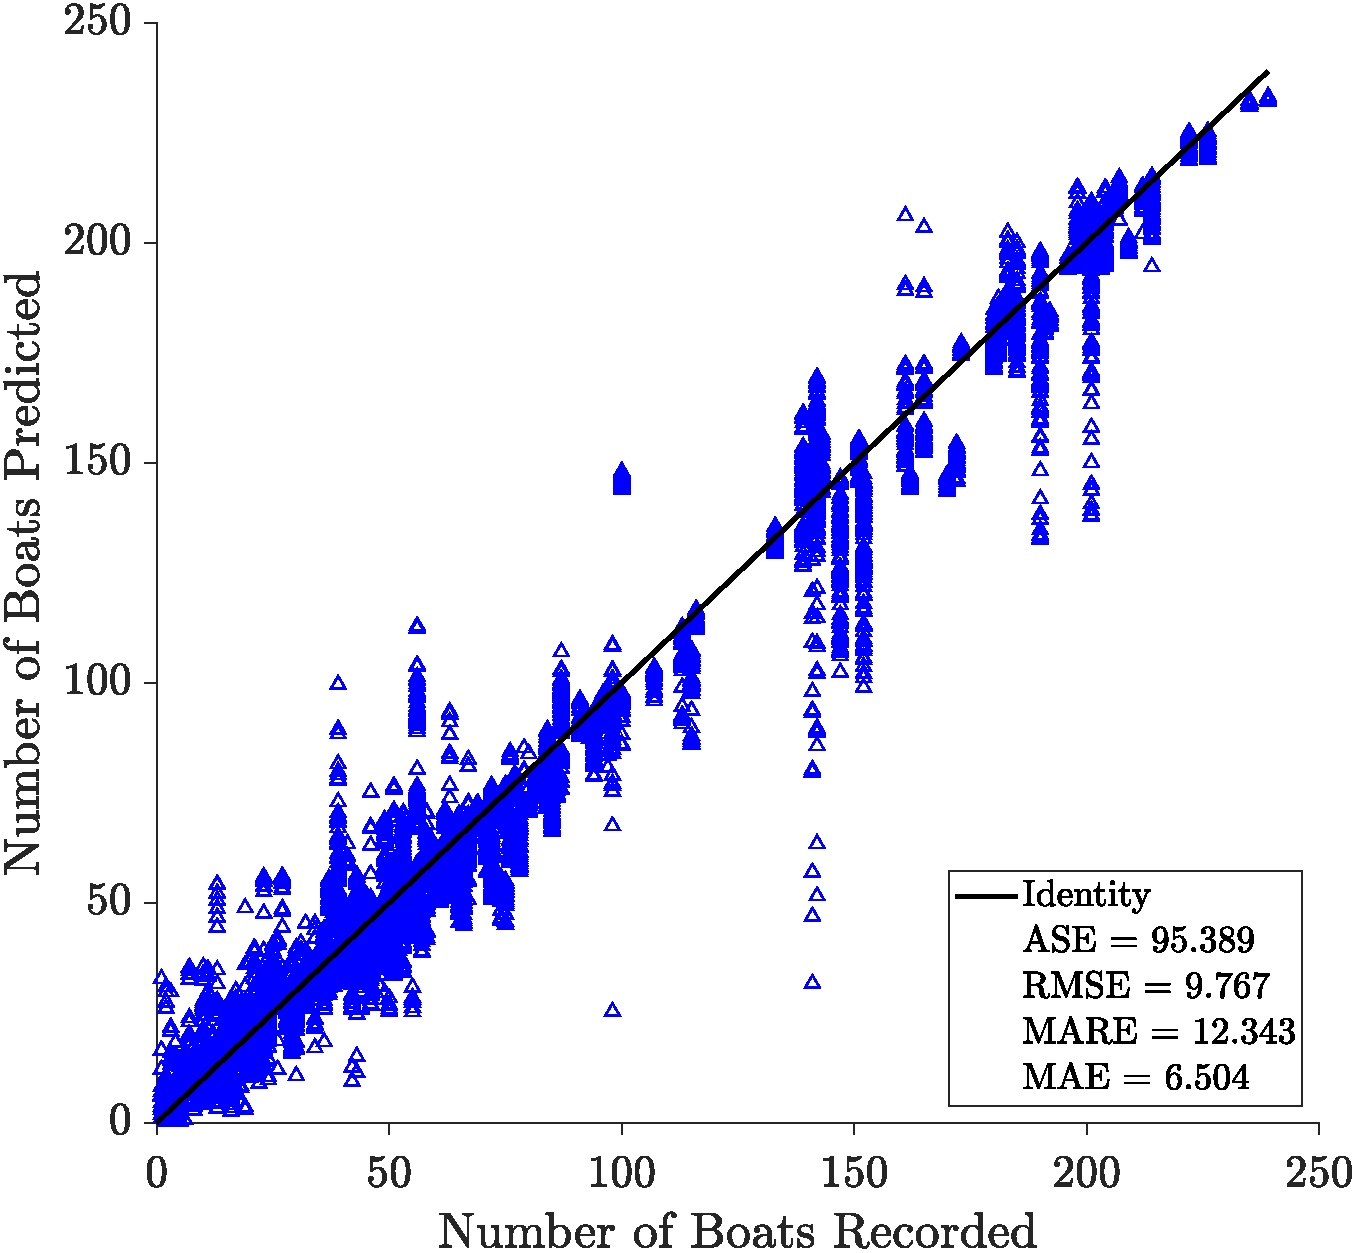
\includegraphics[width=0.65\linewidth]{figures/24-15-1.pdf}
	\caption{Recorded boat traffic versus predicted boat traffic for Model 1.} 
	\label{fig:MOD1}
\end{figure}
%
\begin{figure}
	\centering
	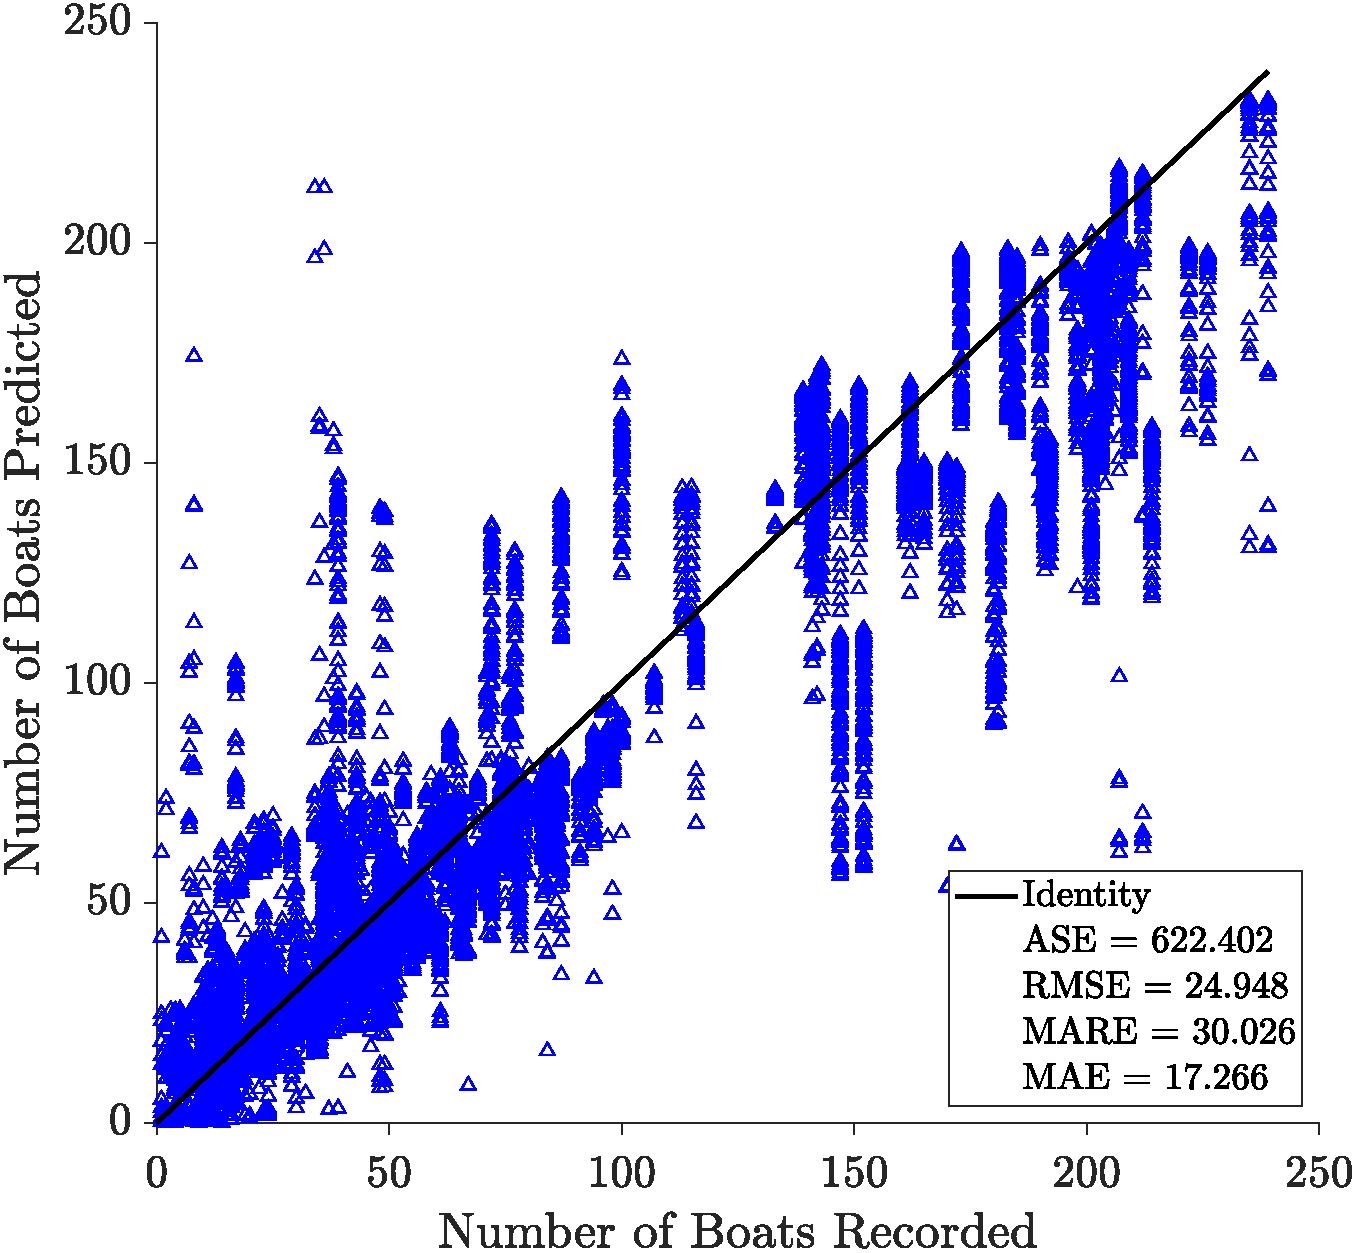
\includegraphics[width=0.65\linewidth]{figures/16-15-1.pdf}
	\caption{Recorded boat traffic versus predicted boat traffic for Model 2.} 
	\label{fig:MOD2}
\end{figure}
%
\begin{figure}
	\centering
	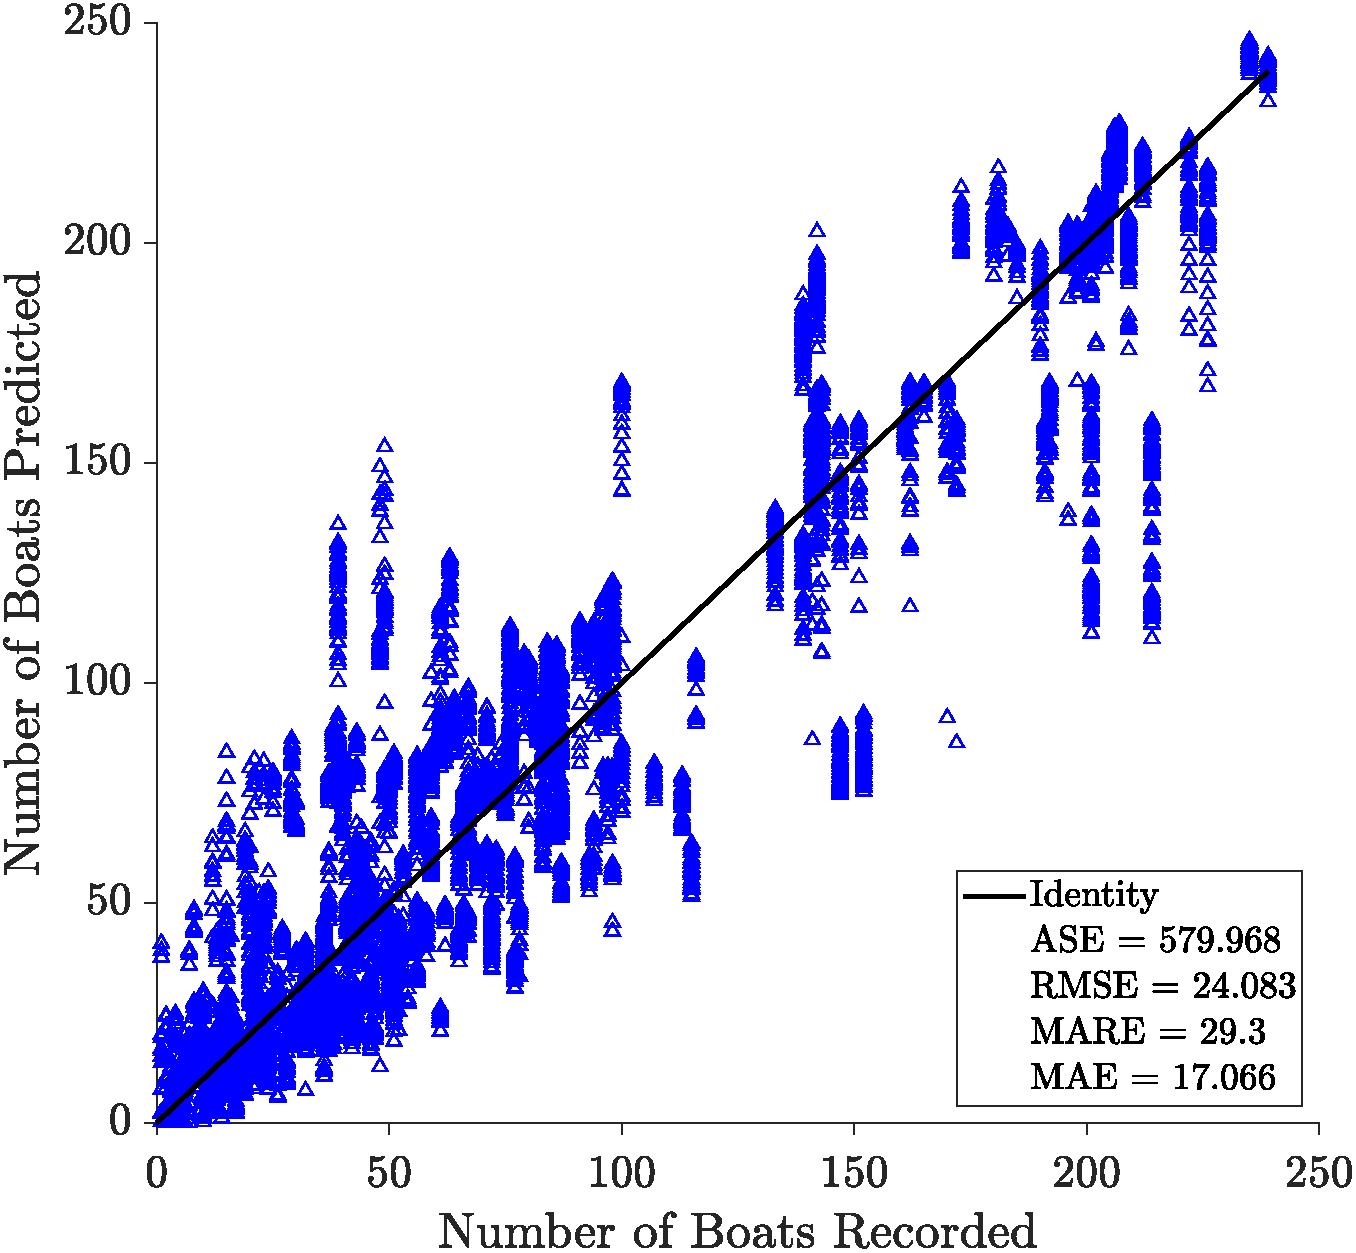
\includegraphics[width=0.65\linewidth]{figures/19-15-1.pdf}
	\caption{Recorded boat traffic versus predicted boat traffic for Model 3.} 
	\label{fig:MOD3}
\end{figure}
%
\begin{figure}
	\centering
	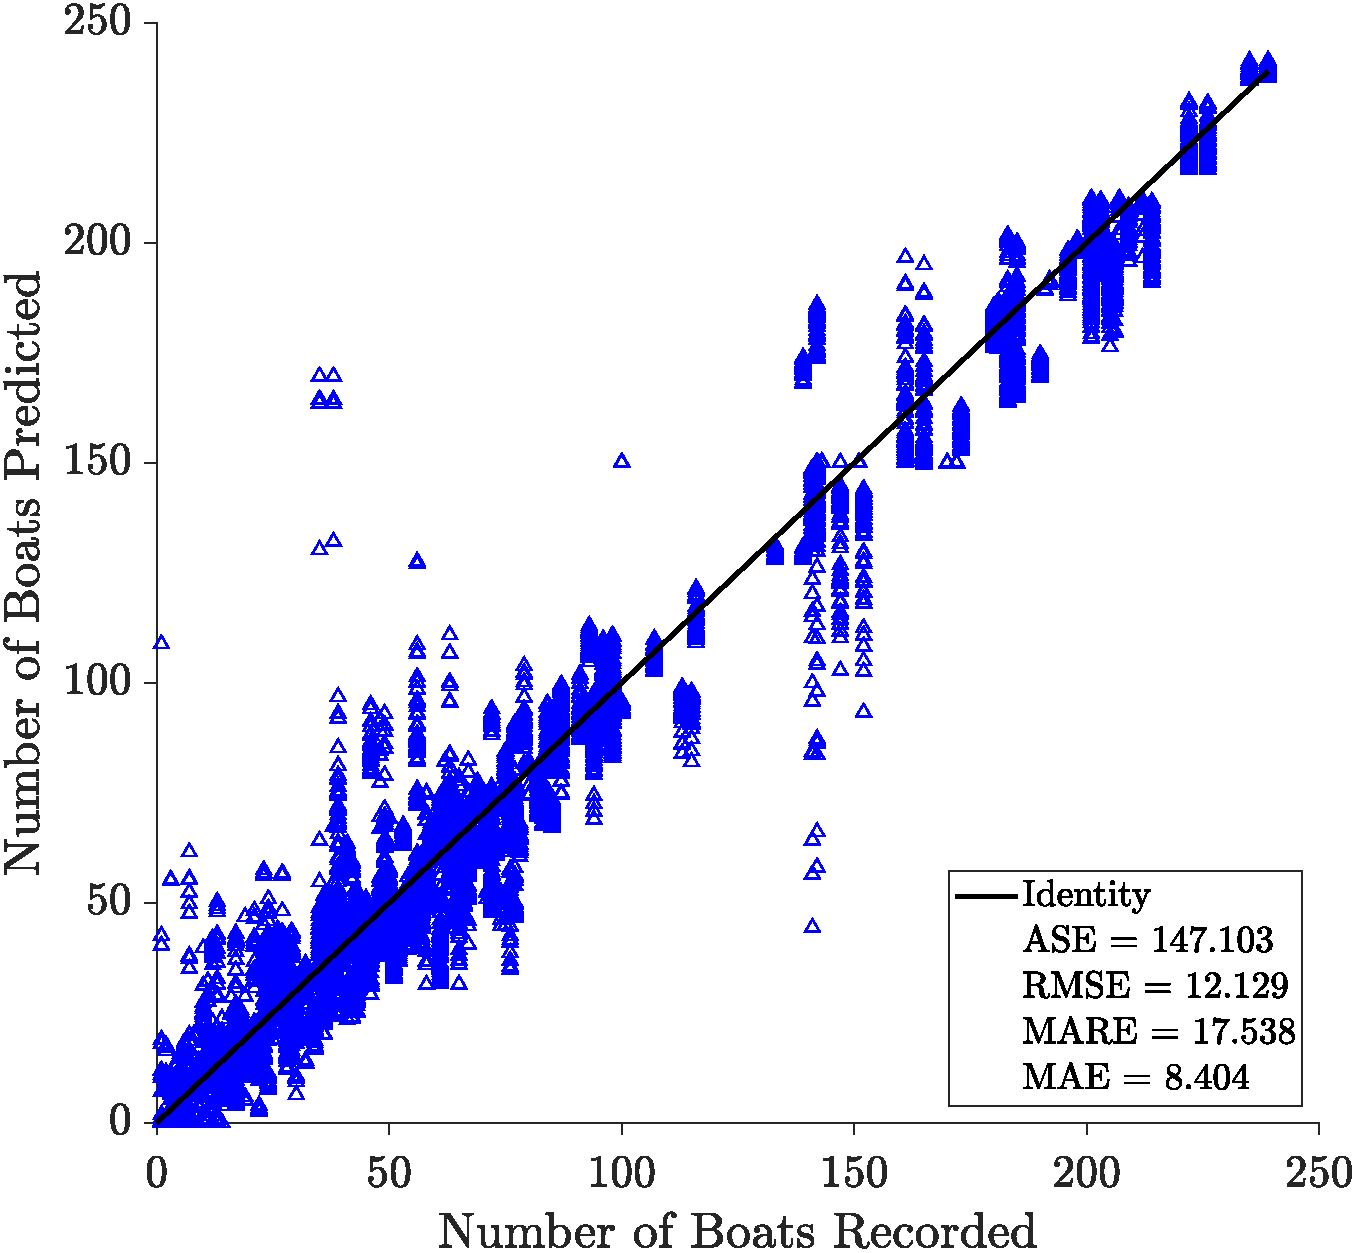
\includegraphics[width=0.65\linewidth]{figures/21-15-1.pdf}
	\caption{Recorded boat traffic versus predicted boat traffic for Model 4.} 
	\label{fig:MOD4}
\end{figure}
%
\begin{figure}
	\centering
	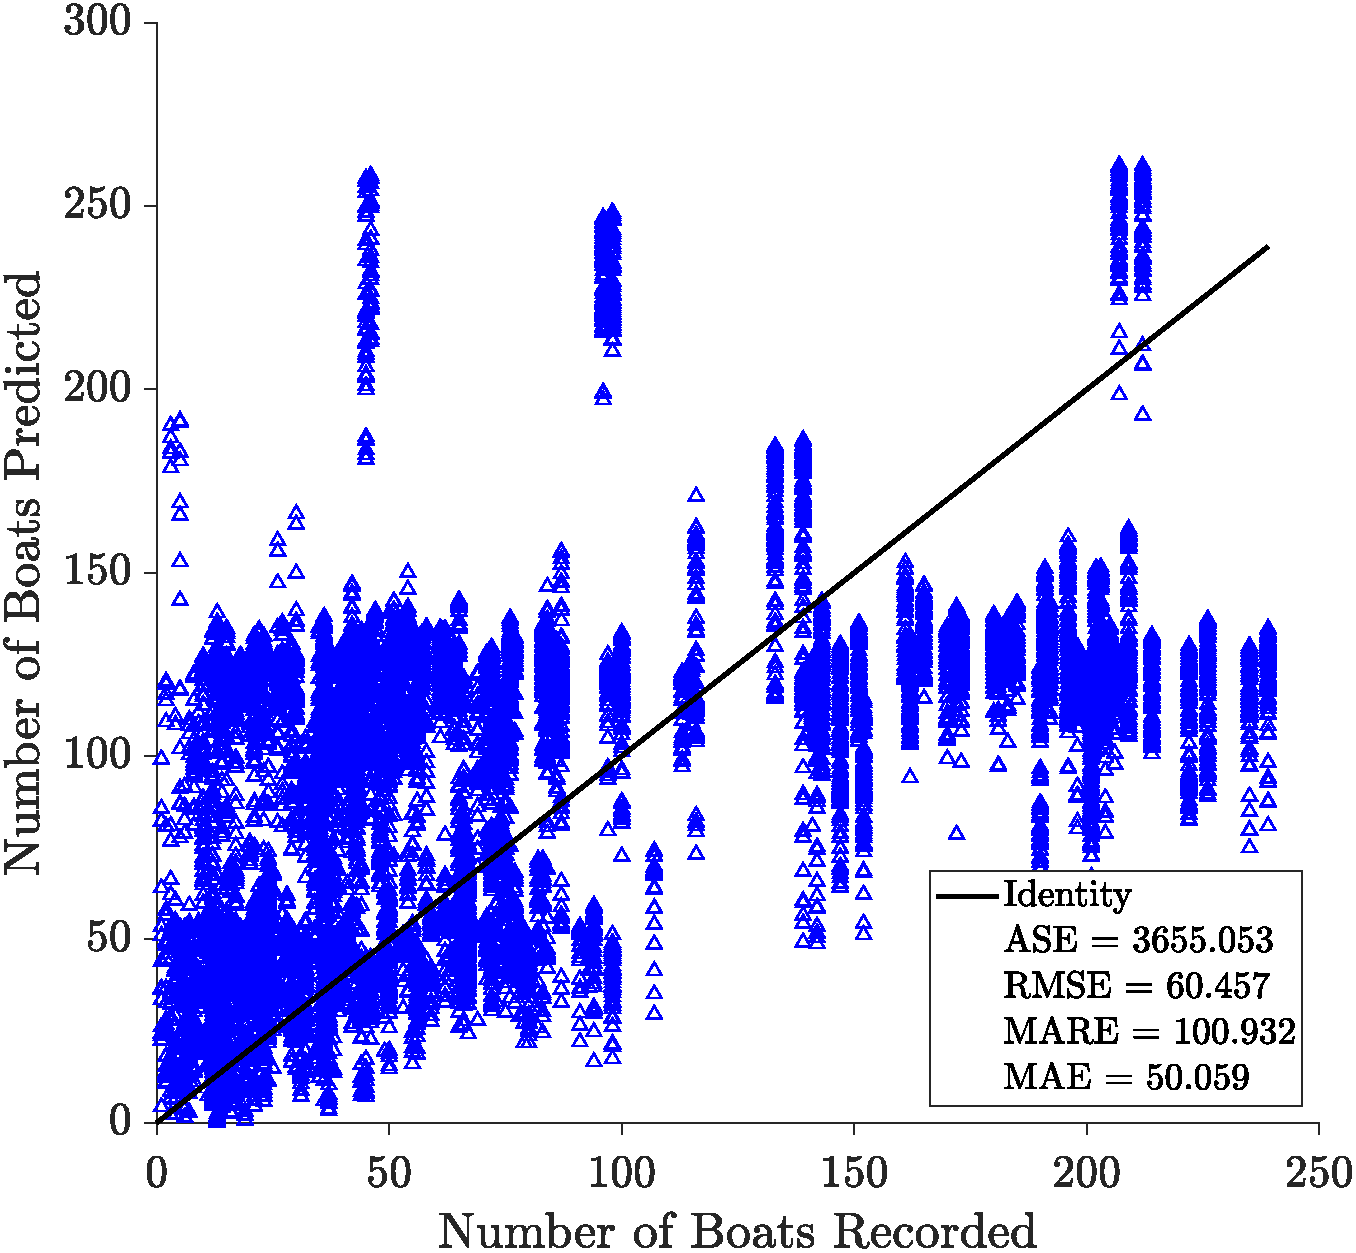
\includegraphics[width=0.65\linewidth]{figures/8-10-1.pdf}
	\caption{Recorded boat traffic versus predicted boat traffic for Model 5.} 
	\label{fig:MOD5}
\end{figure}
%
\begin{figure}
	\centering
	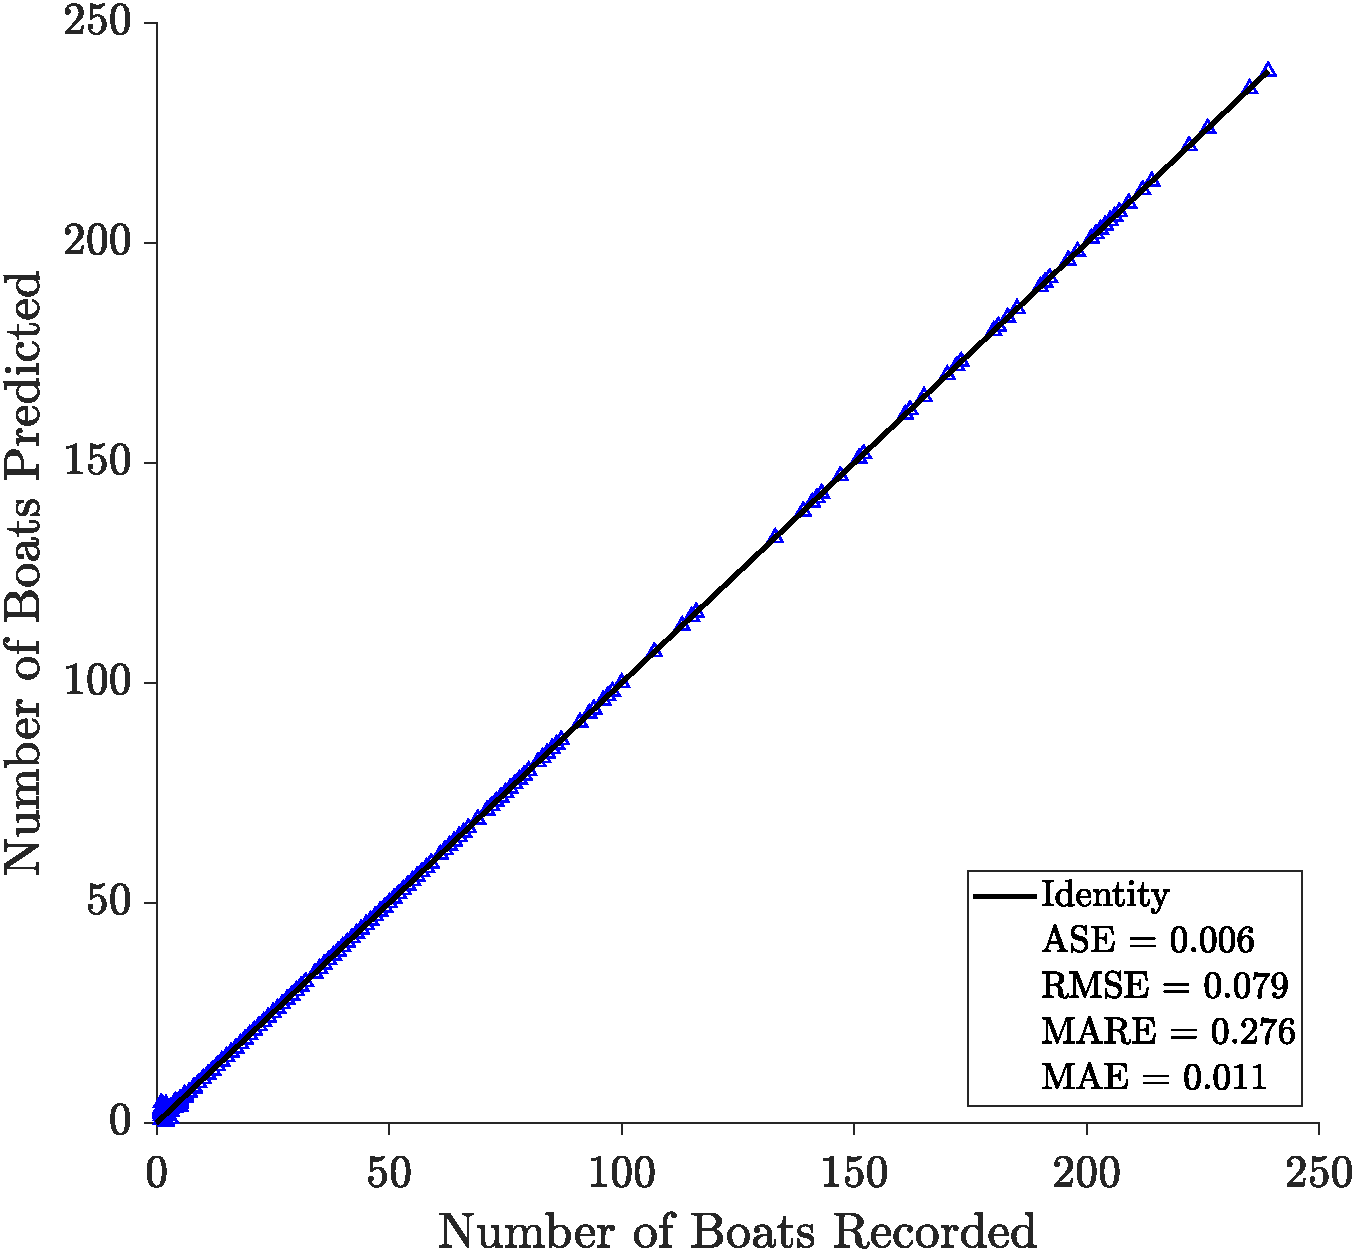
\includegraphics[width=0.65\linewidth]{figures/55-15-1.pdf}
	\caption{Recorded boat traffic versus predicted boat traffic for Model 6.} 
	\label{fig:MOD6}
\end{figure}
%
\begin{figure}
	\centering
	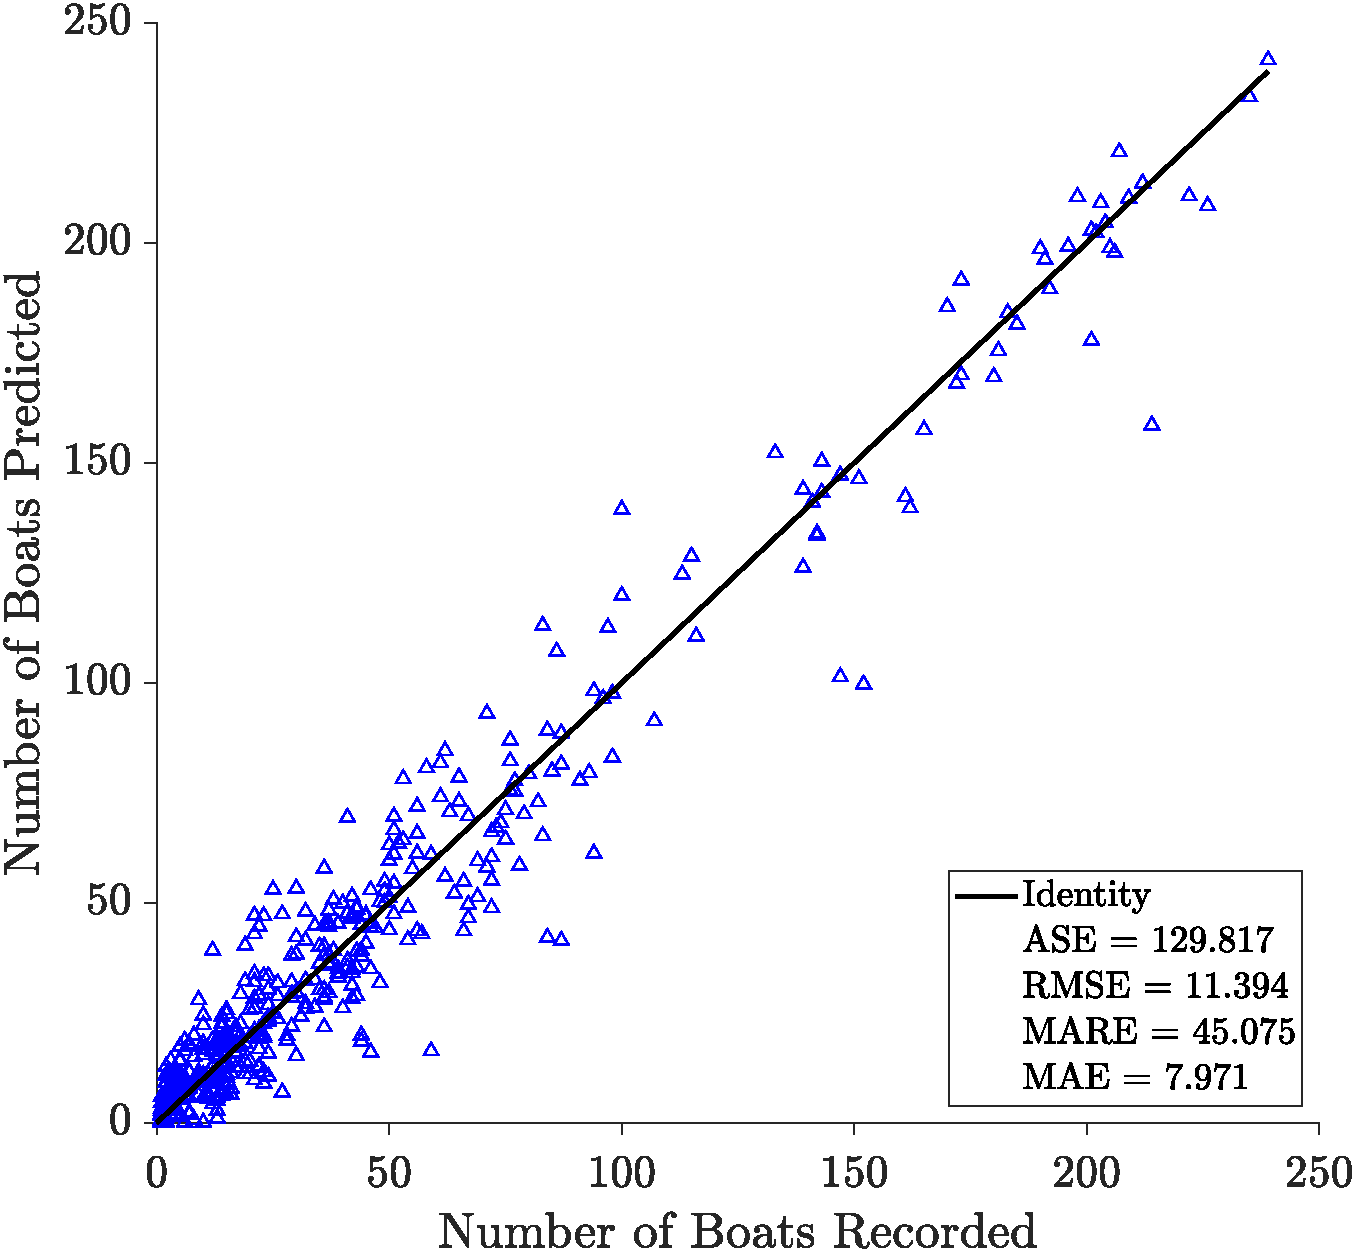
\includegraphics[width=0.65\linewidth]{figures/28-10-1.pdf}
	\caption{Recorded boat traffic versus predicted boat traffic for Model 7.} 
	\label{fig:MOD7}
\end{figure}
%
\begin{figure}
	\centering
	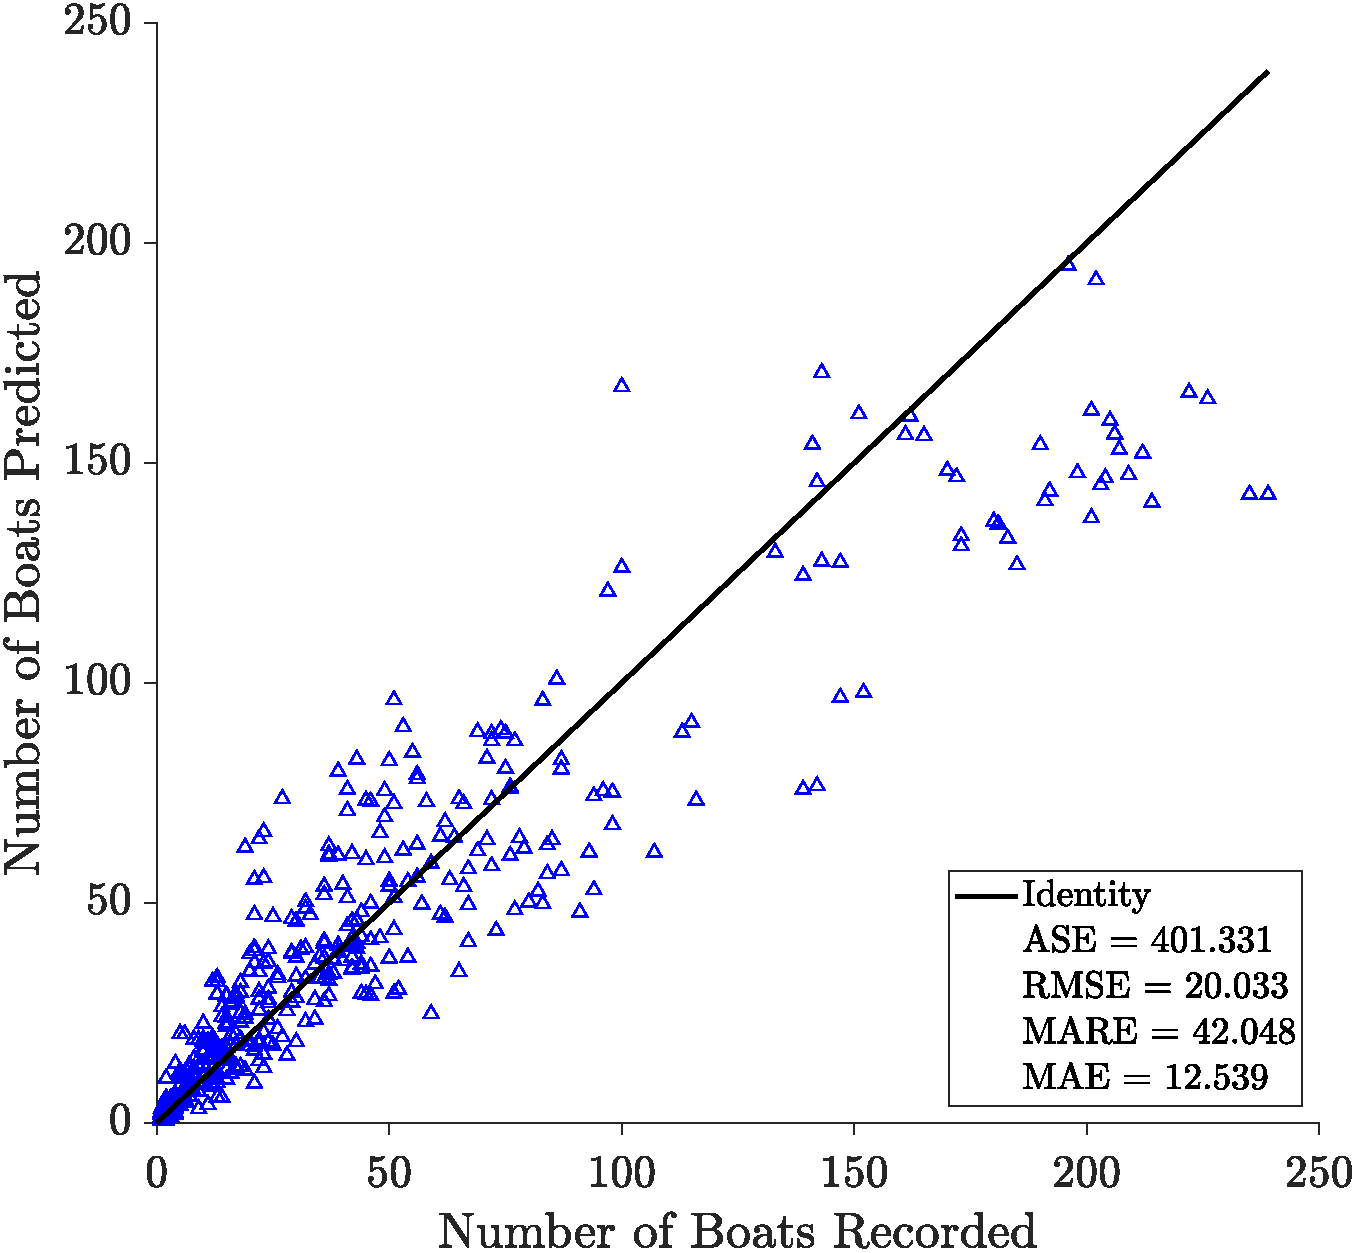
\includegraphics[width=0.65\linewidth]{figures/13-9-1.pdf}
	\caption{Recorded boat traffic versus predicted boat traffic for Model 8.} 
	\label{fig:MOD8}
\end{figure}

\begin{figure}[h!]
	\centering
	\begin{subfigure}[t]{0.49\linewidth}
		\centering
		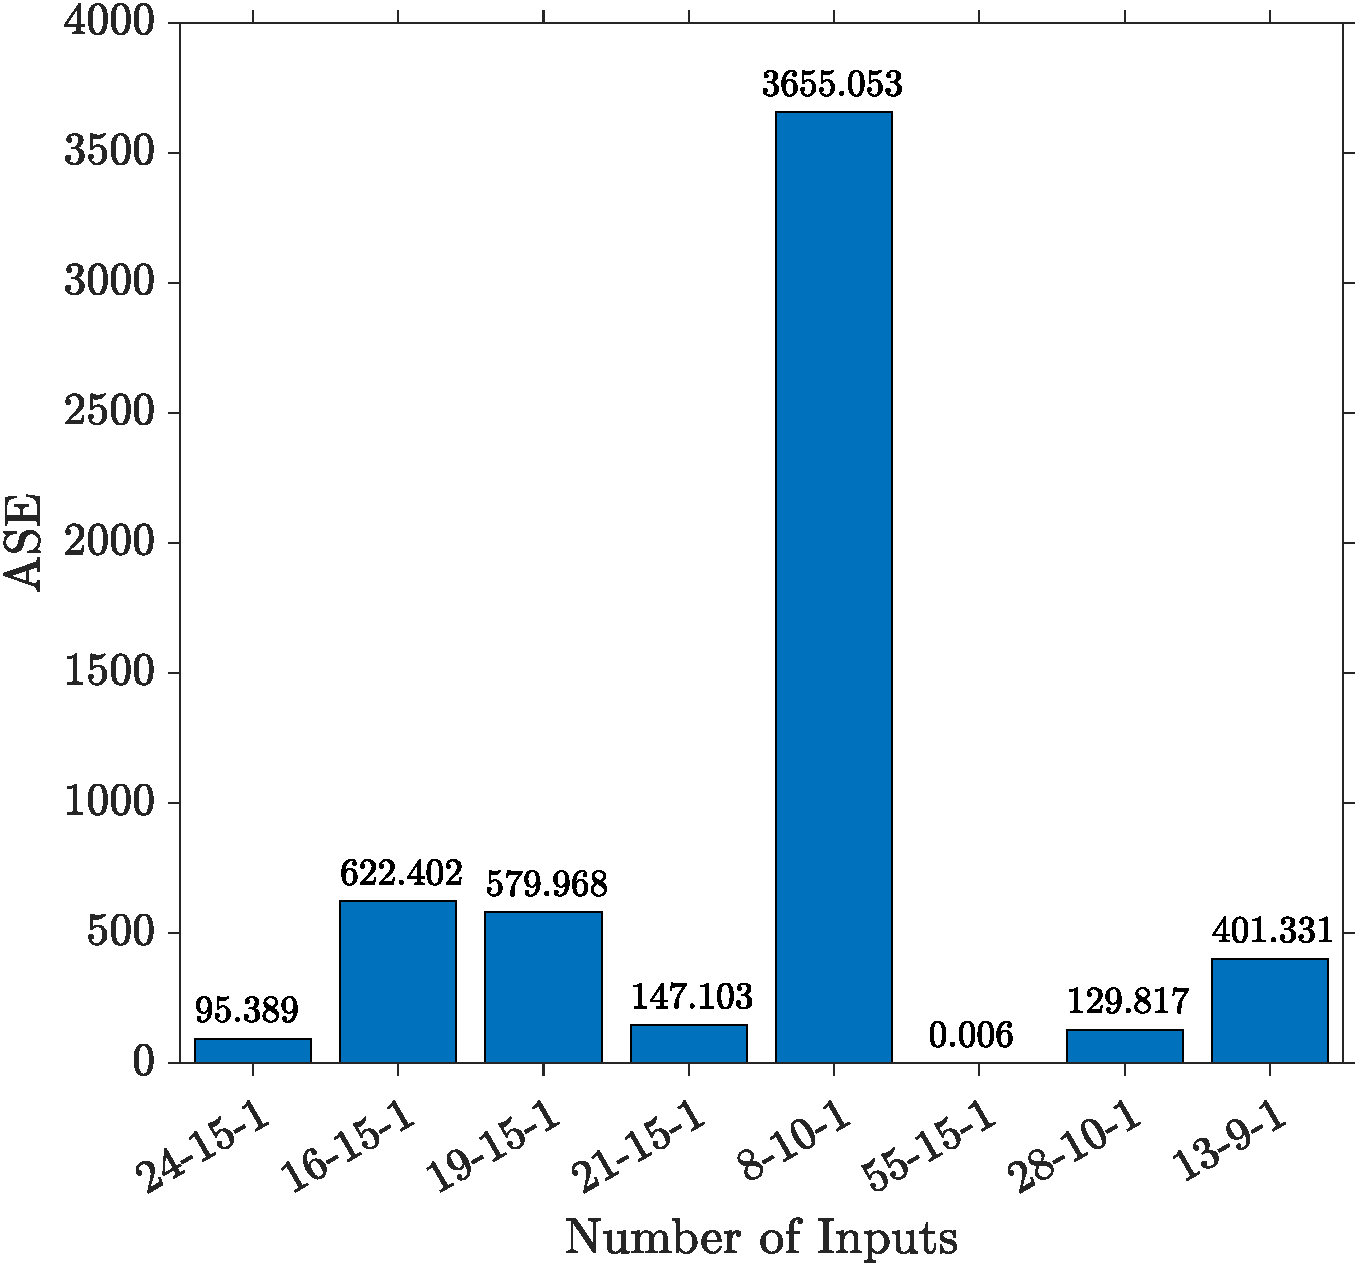
\includegraphics[width=\linewidth]{figures/ASE.pdf}
		\caption{Average-squared-error of models.} 
		\label{fig:ASE}
	\end{subfigure}
	%
	\begin{subfigure}[t]{0.49\linewidth}
		\centering
		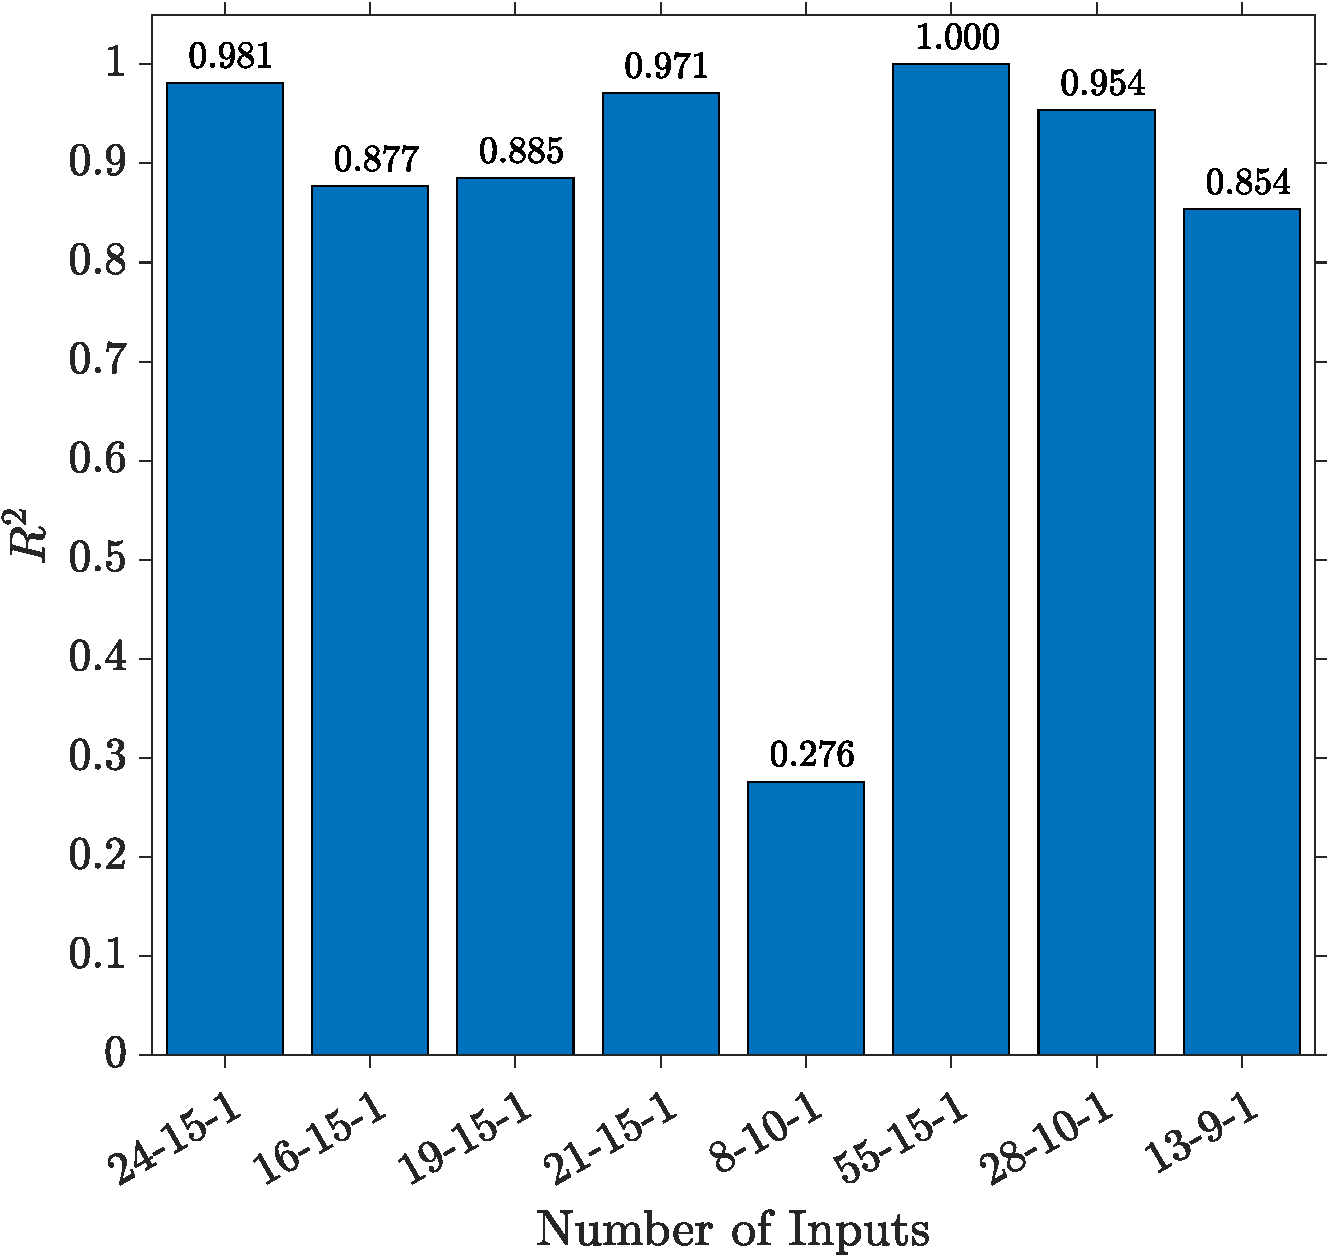
\includegraphics[width=\linewidth]{figures/RSquared.pdf}
		\caption{Coefficient-of-determination of models.} 
		\label{fig:RSQ}
	\end{subfigure}
	%
	\begin{subfigure}[t]{0.49\linewidth}
		\centering
		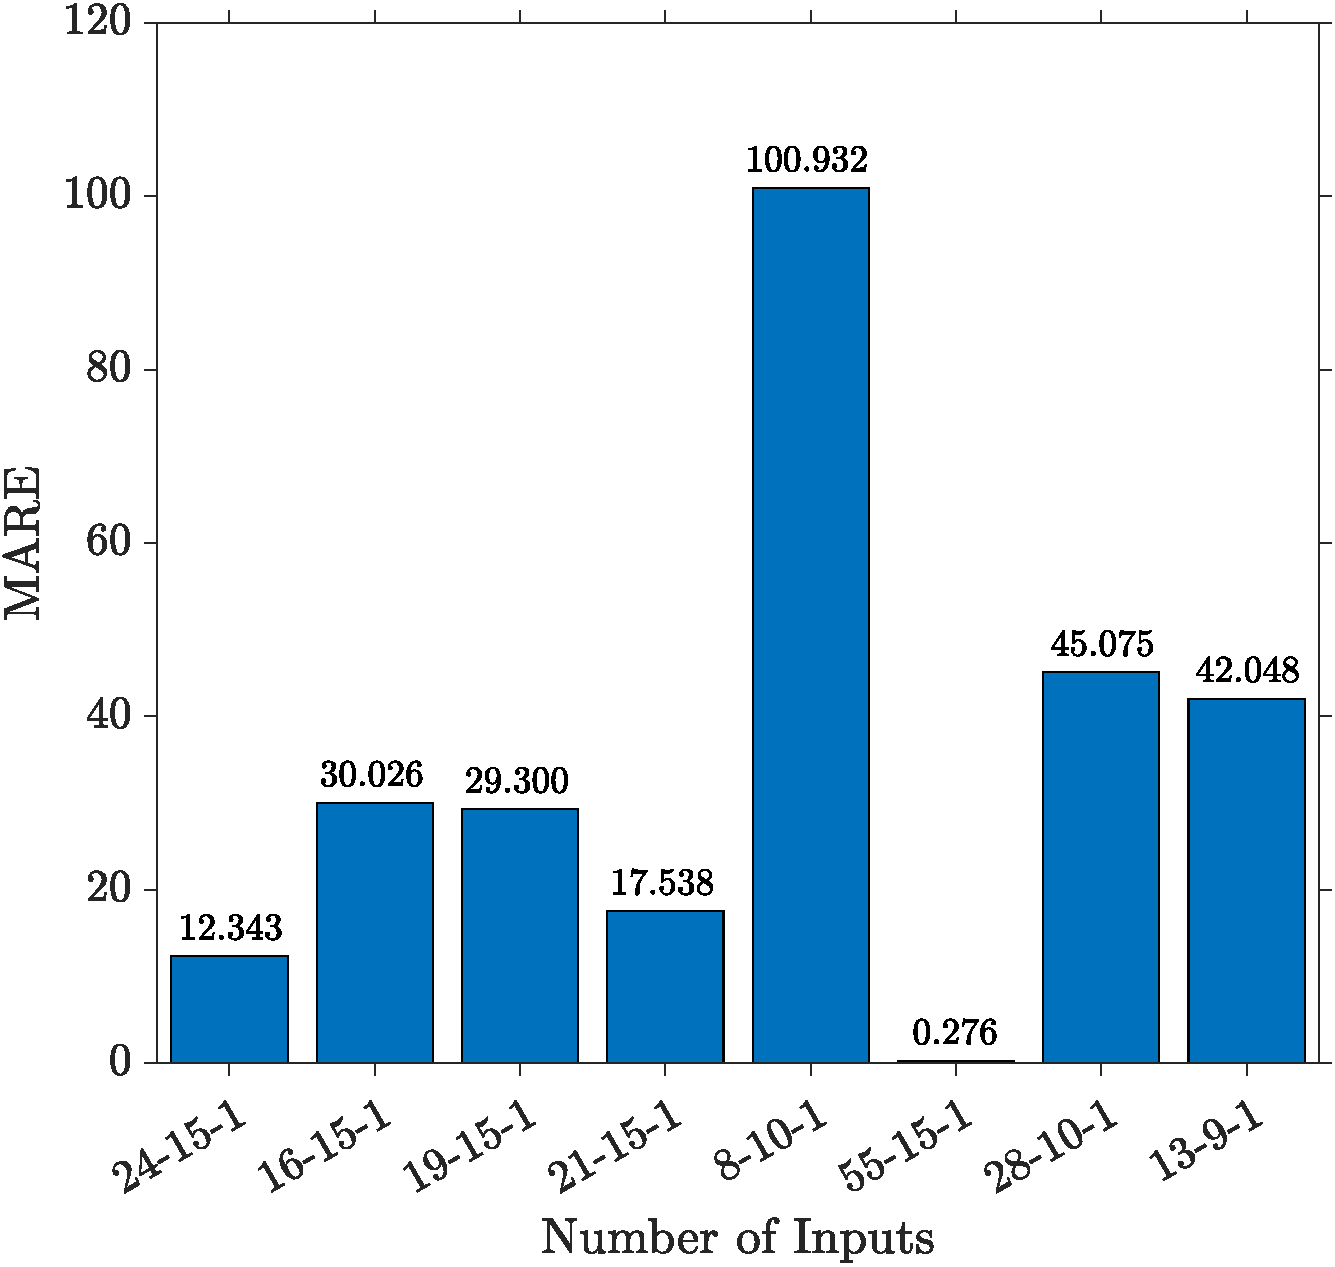
\includegraphics[width=\linewidth]{figures/MARE.pdf}
		\caption{Mean-absolute-relative-error of models.} 
		\label{fig:MARE}
	\end{subfigure}
	%
	\begin{subfigure}[t]{0.49\linewidth}
		\centering
		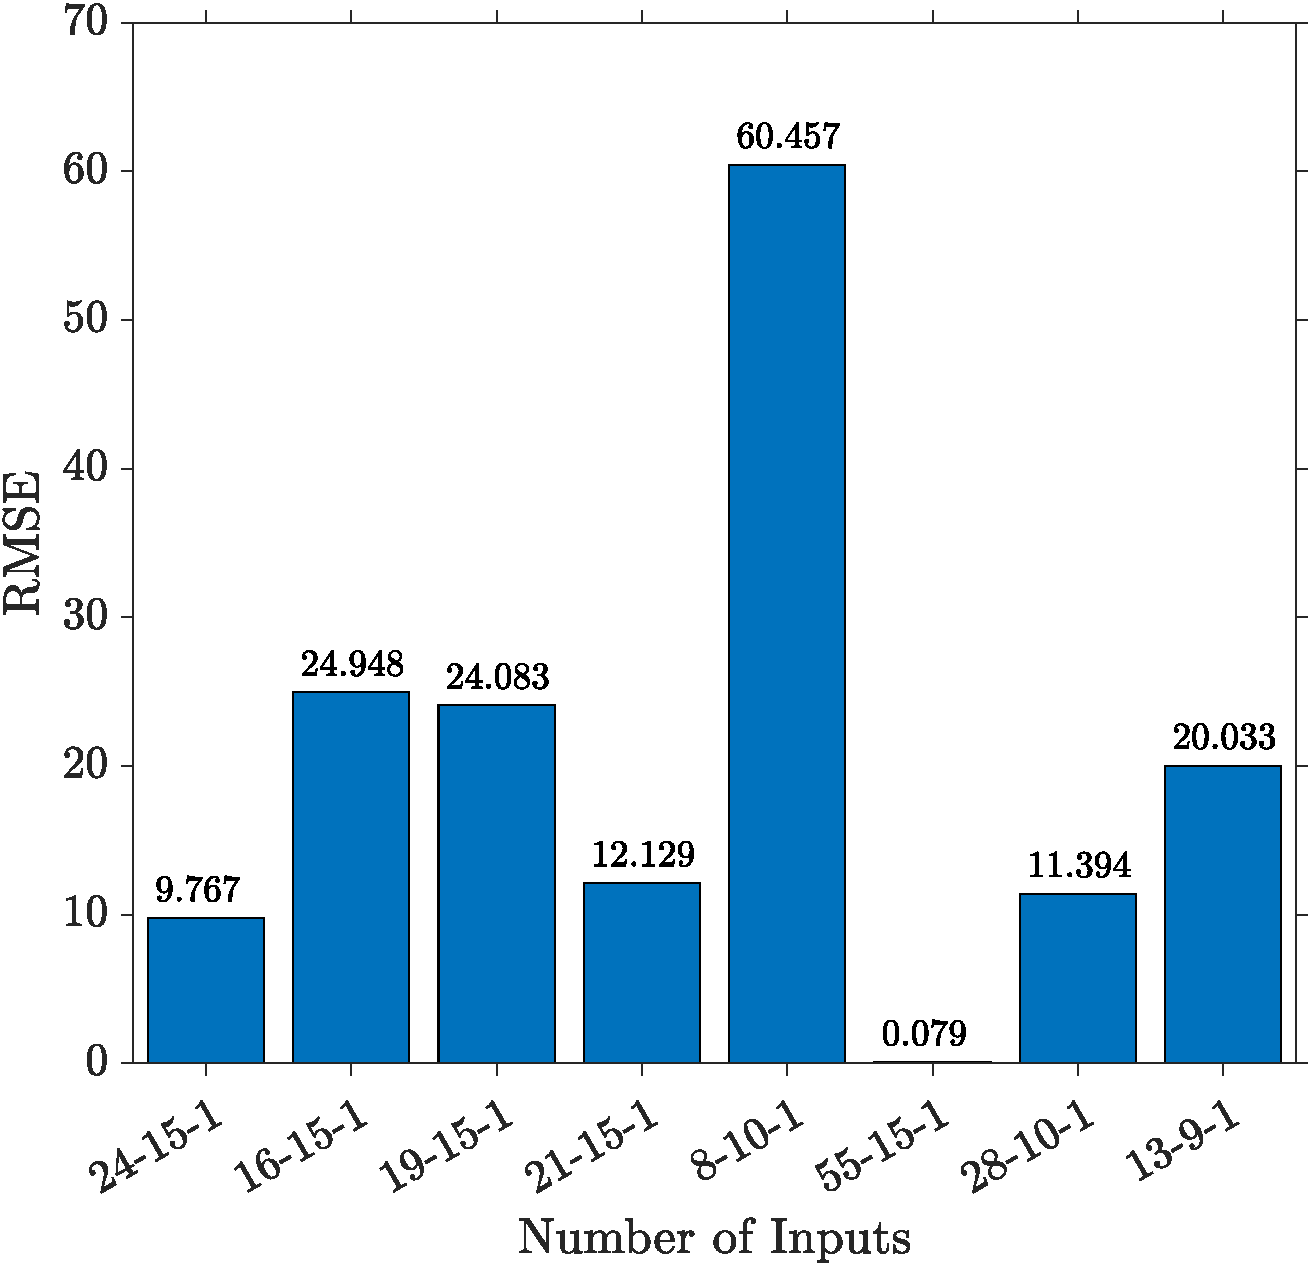
\includegraphics[width=\linewidth]{figures/RMS.pdf}
		\caption{Root-mean-square-errors of models.} 
		\label{fig:RMS}
	\end{subfigure}
	%
	\begin{subfigure}[t]{0.49\linewidth}
		\centering
		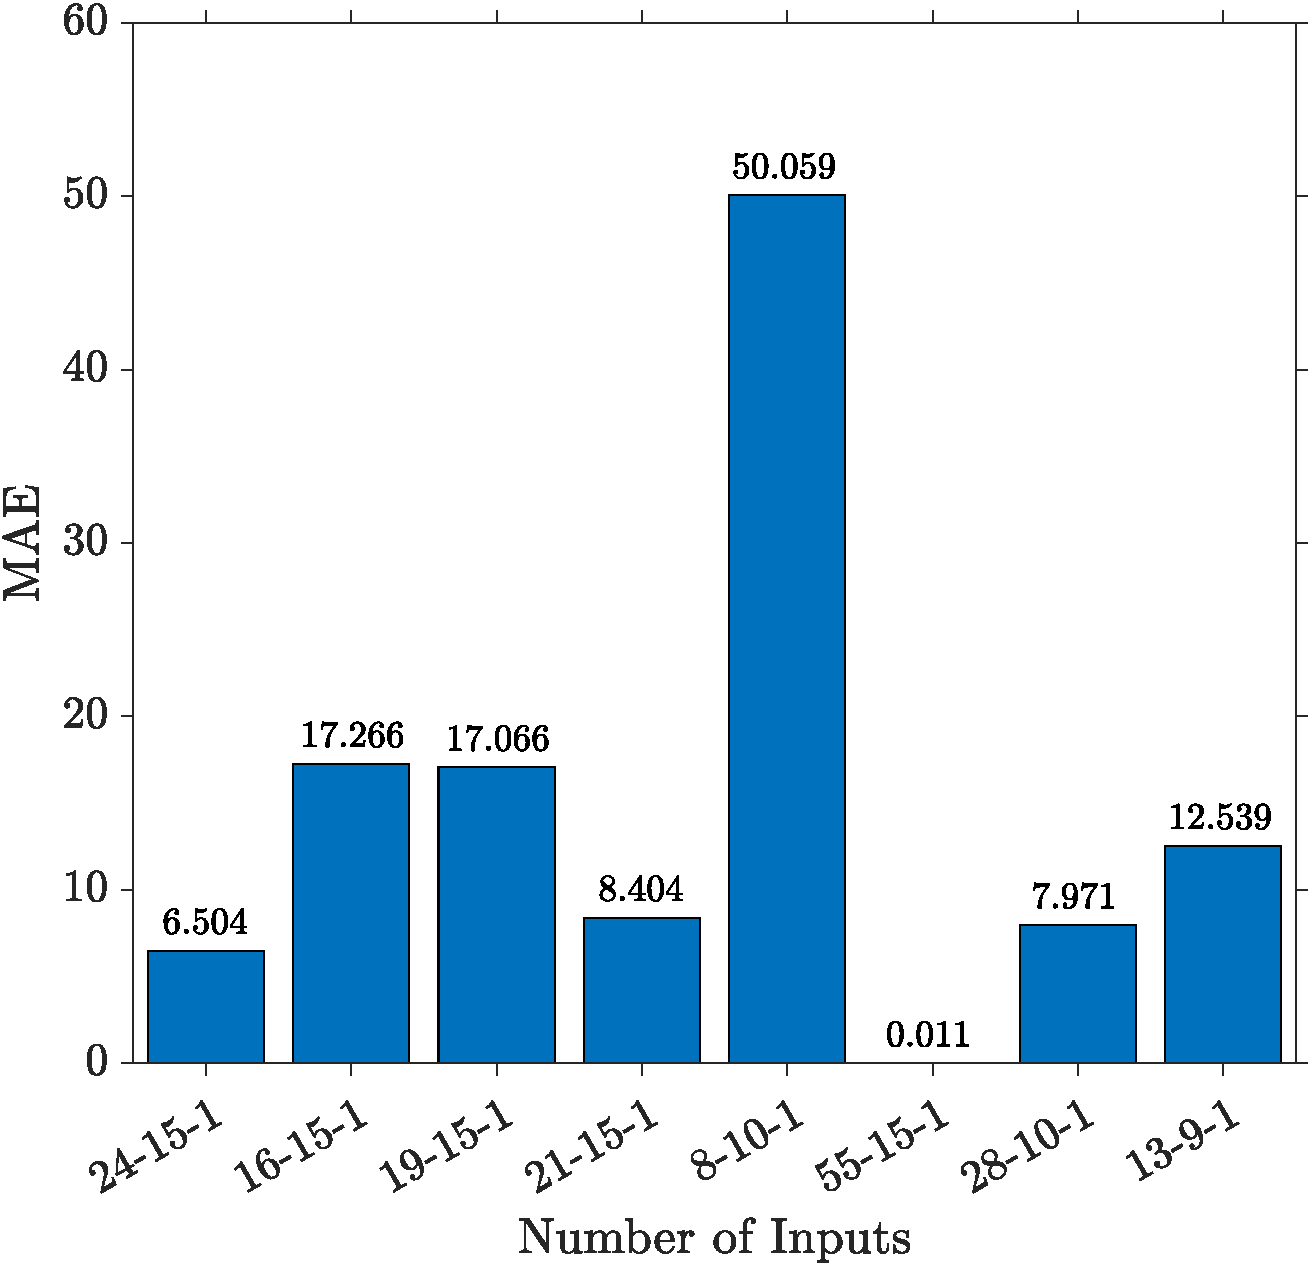
\includegraphics[width=\linewidth]{figures/MAE.pdf}
		\caption{Mean-absolute-error of models.} 
		\label{fig:MAE}
	\end{subfigure}
	\caption{Comparisons of different error quantities for the eight final model networks.}
	\label{fig:ERRORS}
\end{figure}

%\begin{figure}[h!]
%	\centering
%	\begin{subfigure}[t]{0.49\linewidth}
%		\centering
%		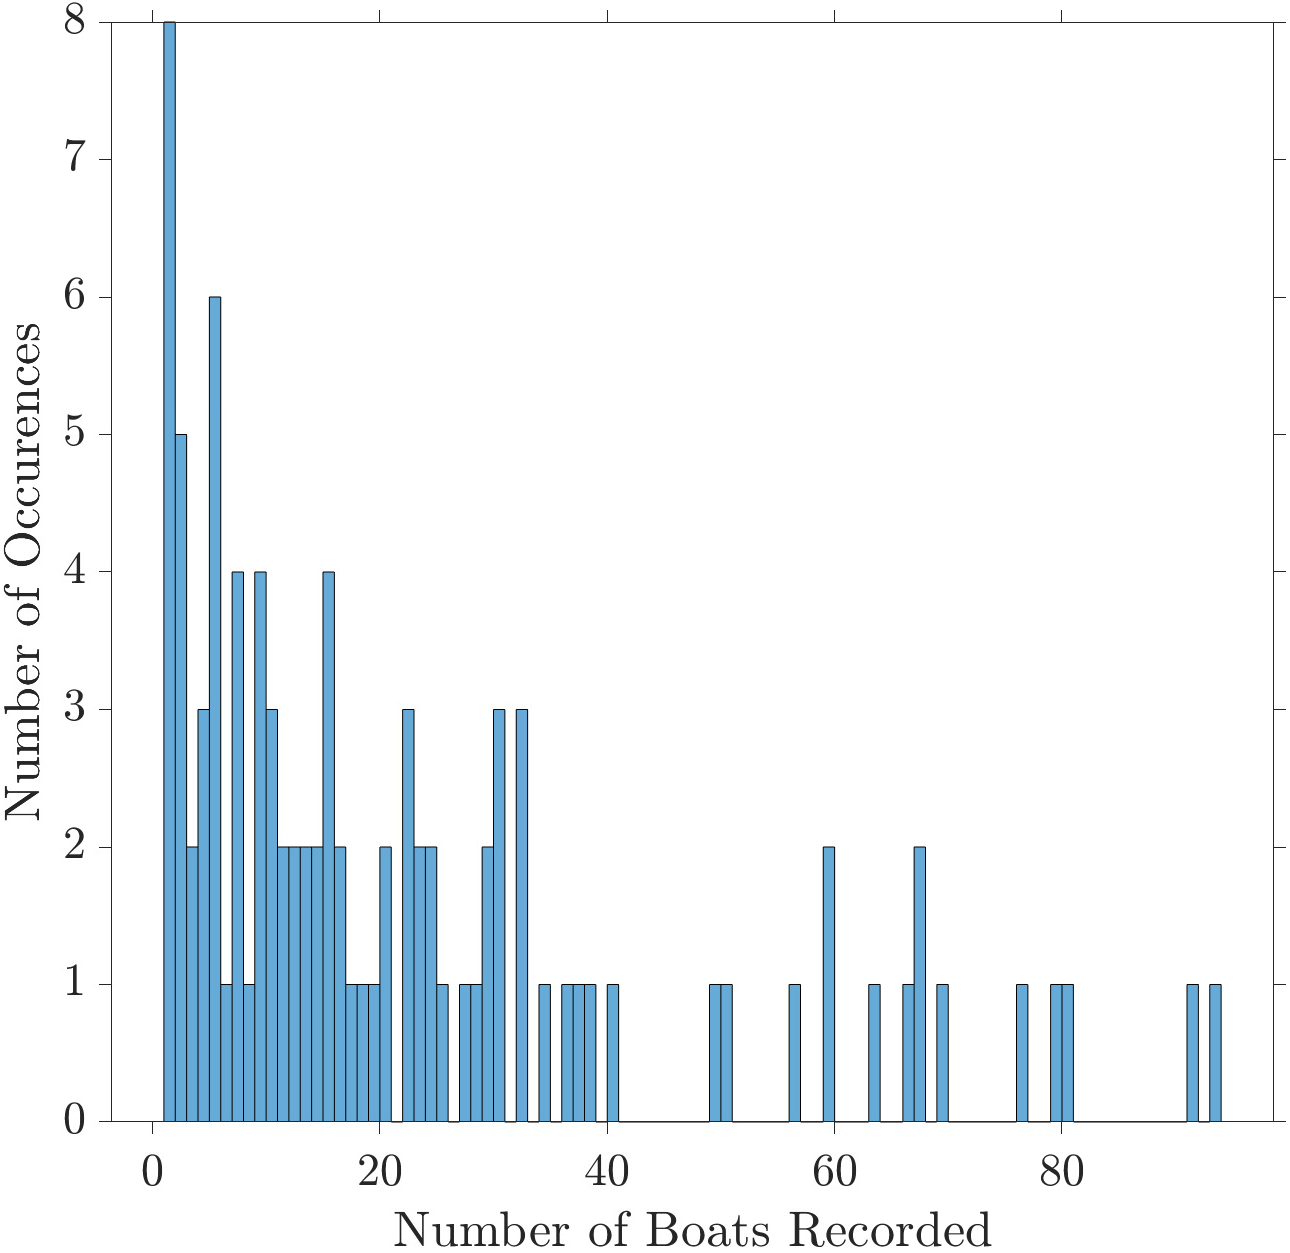
\includegraphics[width=\linewidth]{figures/LOG1.pdf}
%		\caption{Wave Staff 1} 
%		\label{fig:BoatsL1}
%	\end{subfigure}
%	%
%	\begin{subfigure}[t]{0.49\linewidth}
%		\centering
%		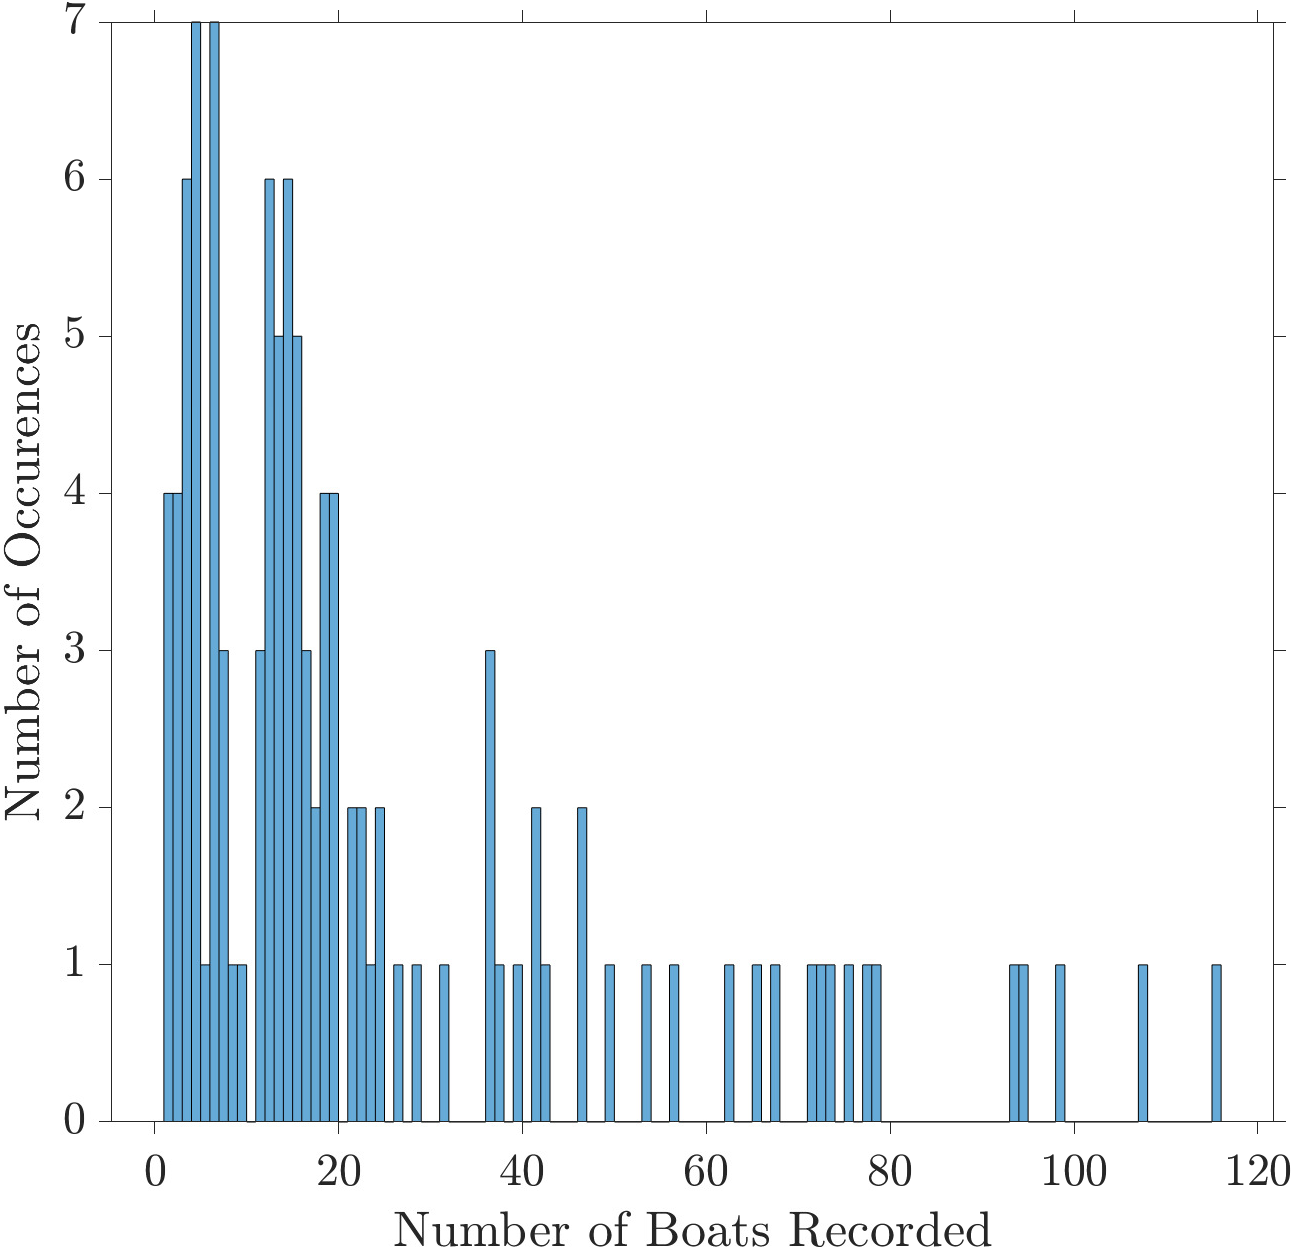
\includegraphics[width=\linewidth]{figures/LOG2.pdf}
%		\caption{Wave Staff 2} 
%		\label{fig:BoatsL2}
%	\end{subfigure}
%	%
%	\begin{subfigure}[t]{0.49\linewidth}
%		\centering
%		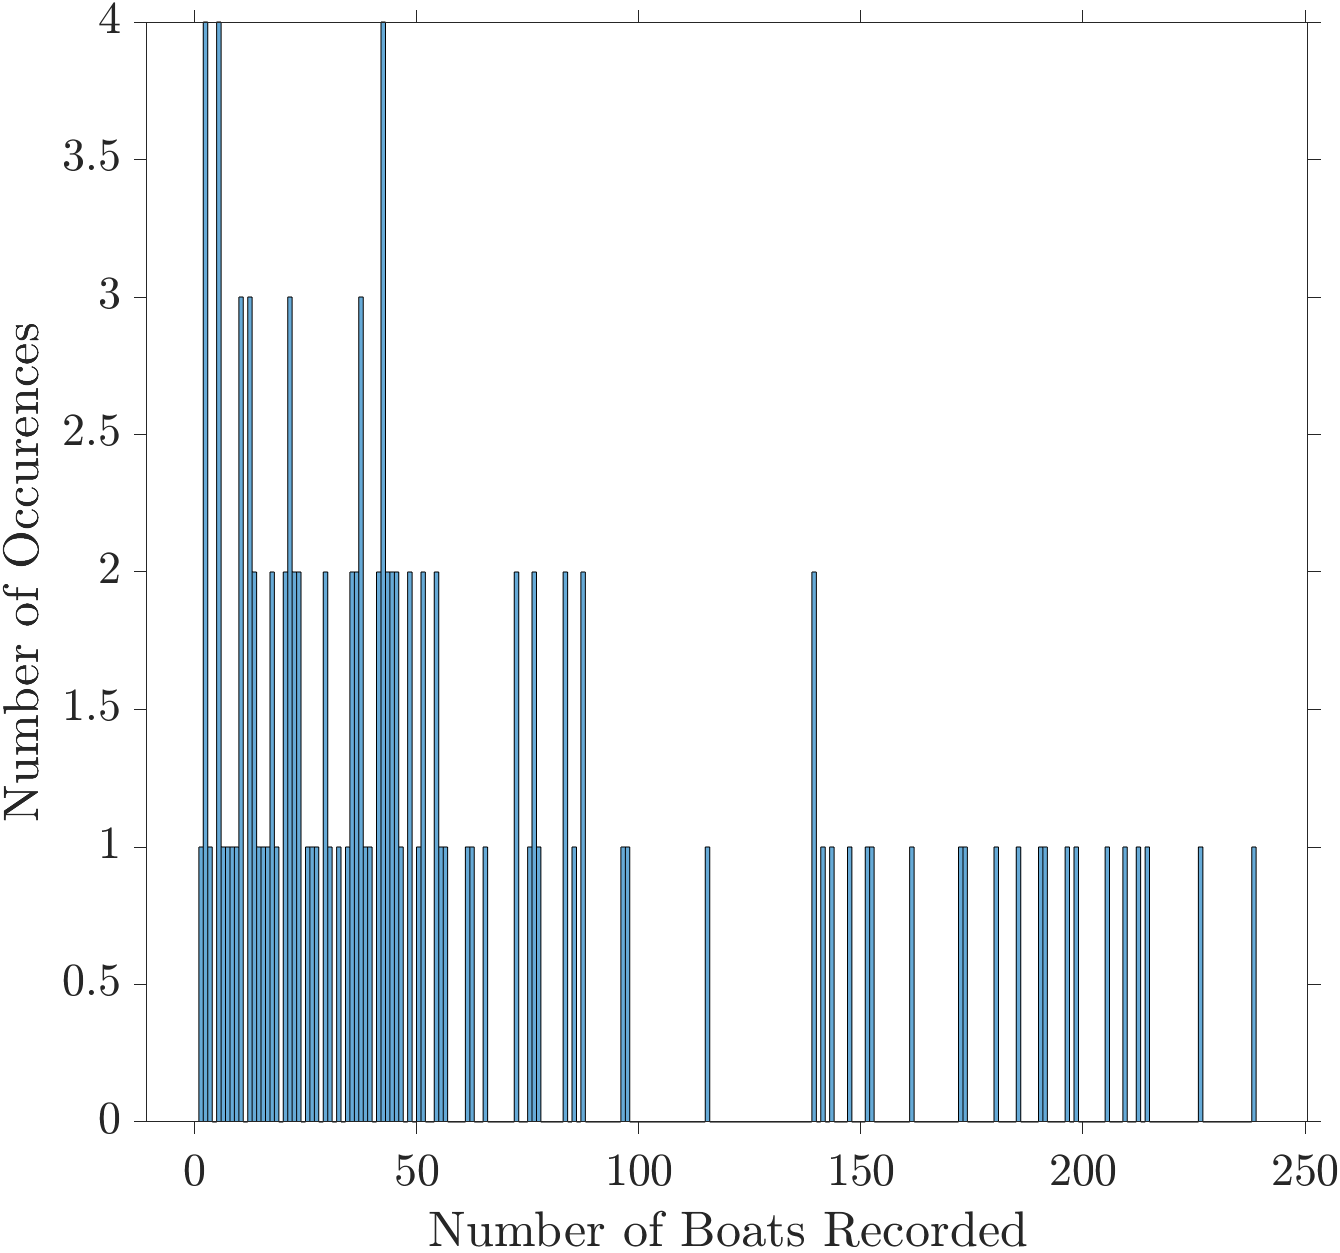
\includegraphics[width=\linewidth]{figures/LOG3.pdf}
%		\caption{Wave Staff 3} 
%		\label{fig:BoatsL3}
%	\end{subfigure}
%	%
%	\begin{subfigure}[t]{0.49\linewidth}
%		\centering
%		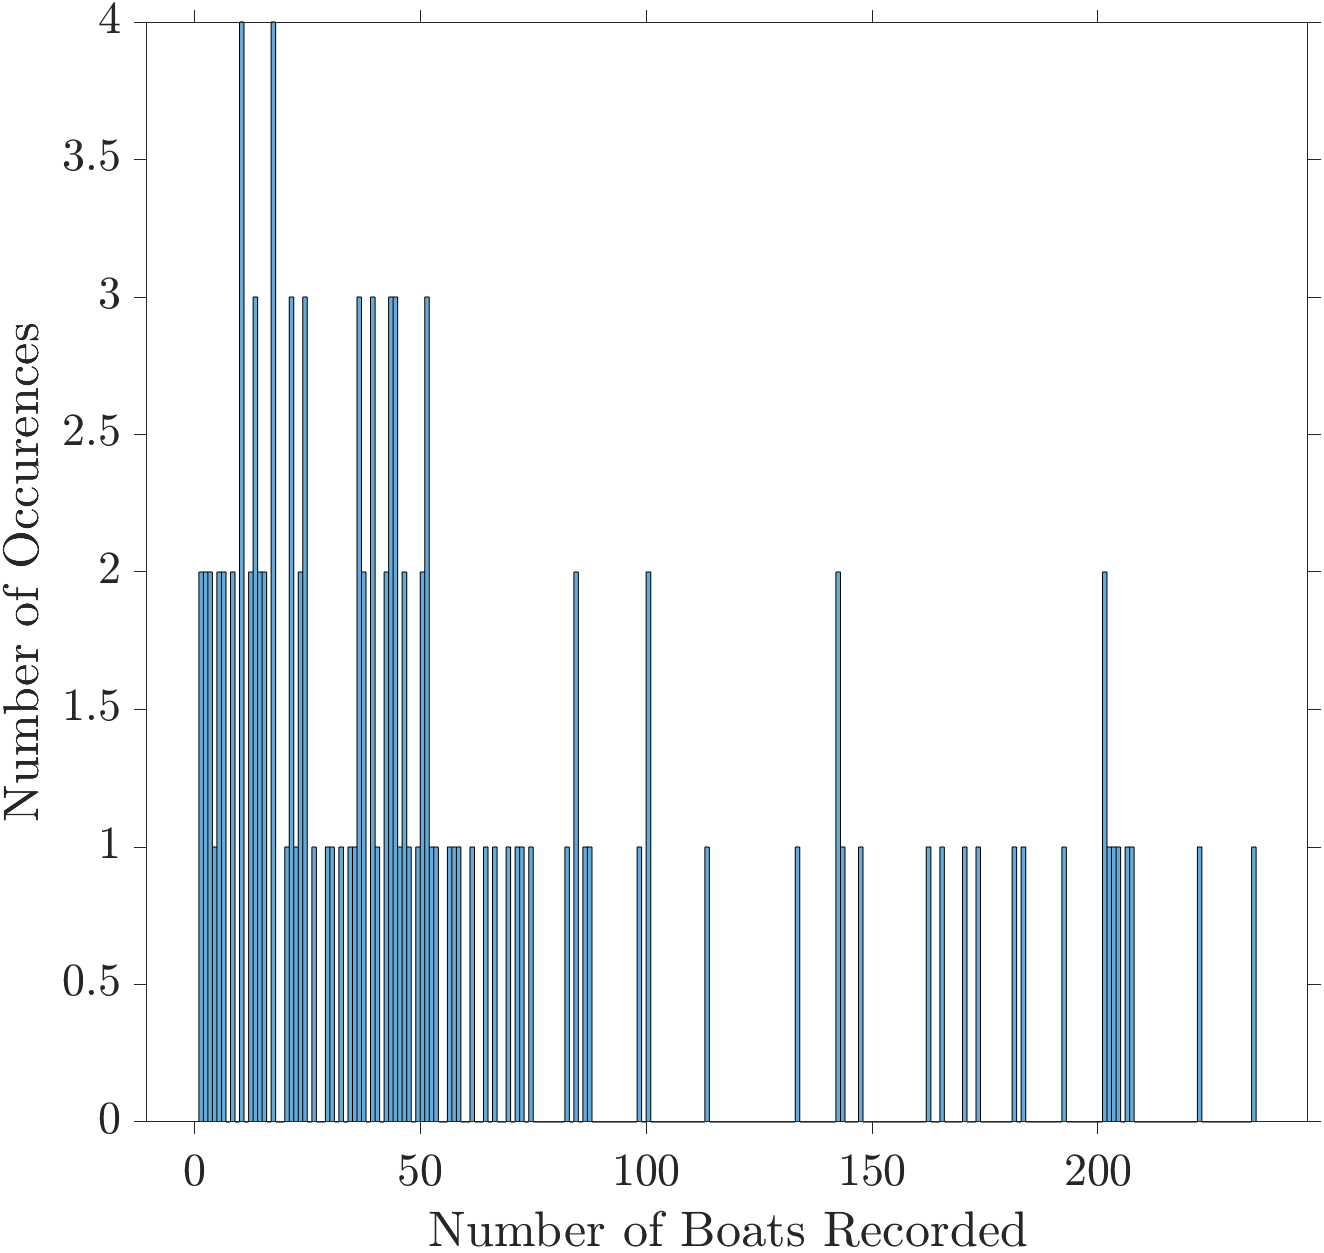
\includegraphics[width=\linewidth]{figures/LOG4.pdf}
%		\caption{Wave Staff 4} 
%		\label{fig:BoatsL4}
%	\end{subfigure}
%	\caption{Histograms of total daily boat traffic recorded at different location.}
%	\label{fig:BoatTraffic}
%\end{figure}
%


\end{document}
